\documentclass[letterpaper]{book}
%permite agregar codigo fuente
\usepackage{listings}
\lstset{language=c++,
		showstringspaces=false,
		 breaklines=true}
\usepackage{graphicx}
\usepackage[bookmarks=true]{hyperref} %add table of contents to the pdf file
\usepackage[spanish]{babel} %español
\usepackage[utf8x]{inputenc} 
%establece los limites de la numeracion de capitulos
\setcounter{secnumdepth}{4}
\setcounter{tocdepth}{4}
\title{UDG\_Create User Guide}
\author{Omar Alejandro Rodr\'{i}guez Rosas}

\begin{document}


\maketitle

\tableofcontents
\chapter{Introduction}


 

\chapter{Setup}

\section{Conexiones físicas}
Para la correcta ejecución de los programas creados con la biblioteca UDG\_Create es necesario realizar algunas conexiones físicas entre los distintos componentes de hardware.\\
1. Conecte el cable DB-25 macho de la placa fenólica al puerto DB-25 hembra en la bahía de carga del Create\textsuperscript{\textregistered} como se muestra en la figura \ref{fig:cargoCable}.\\
\begin{figure}
\begin{center}
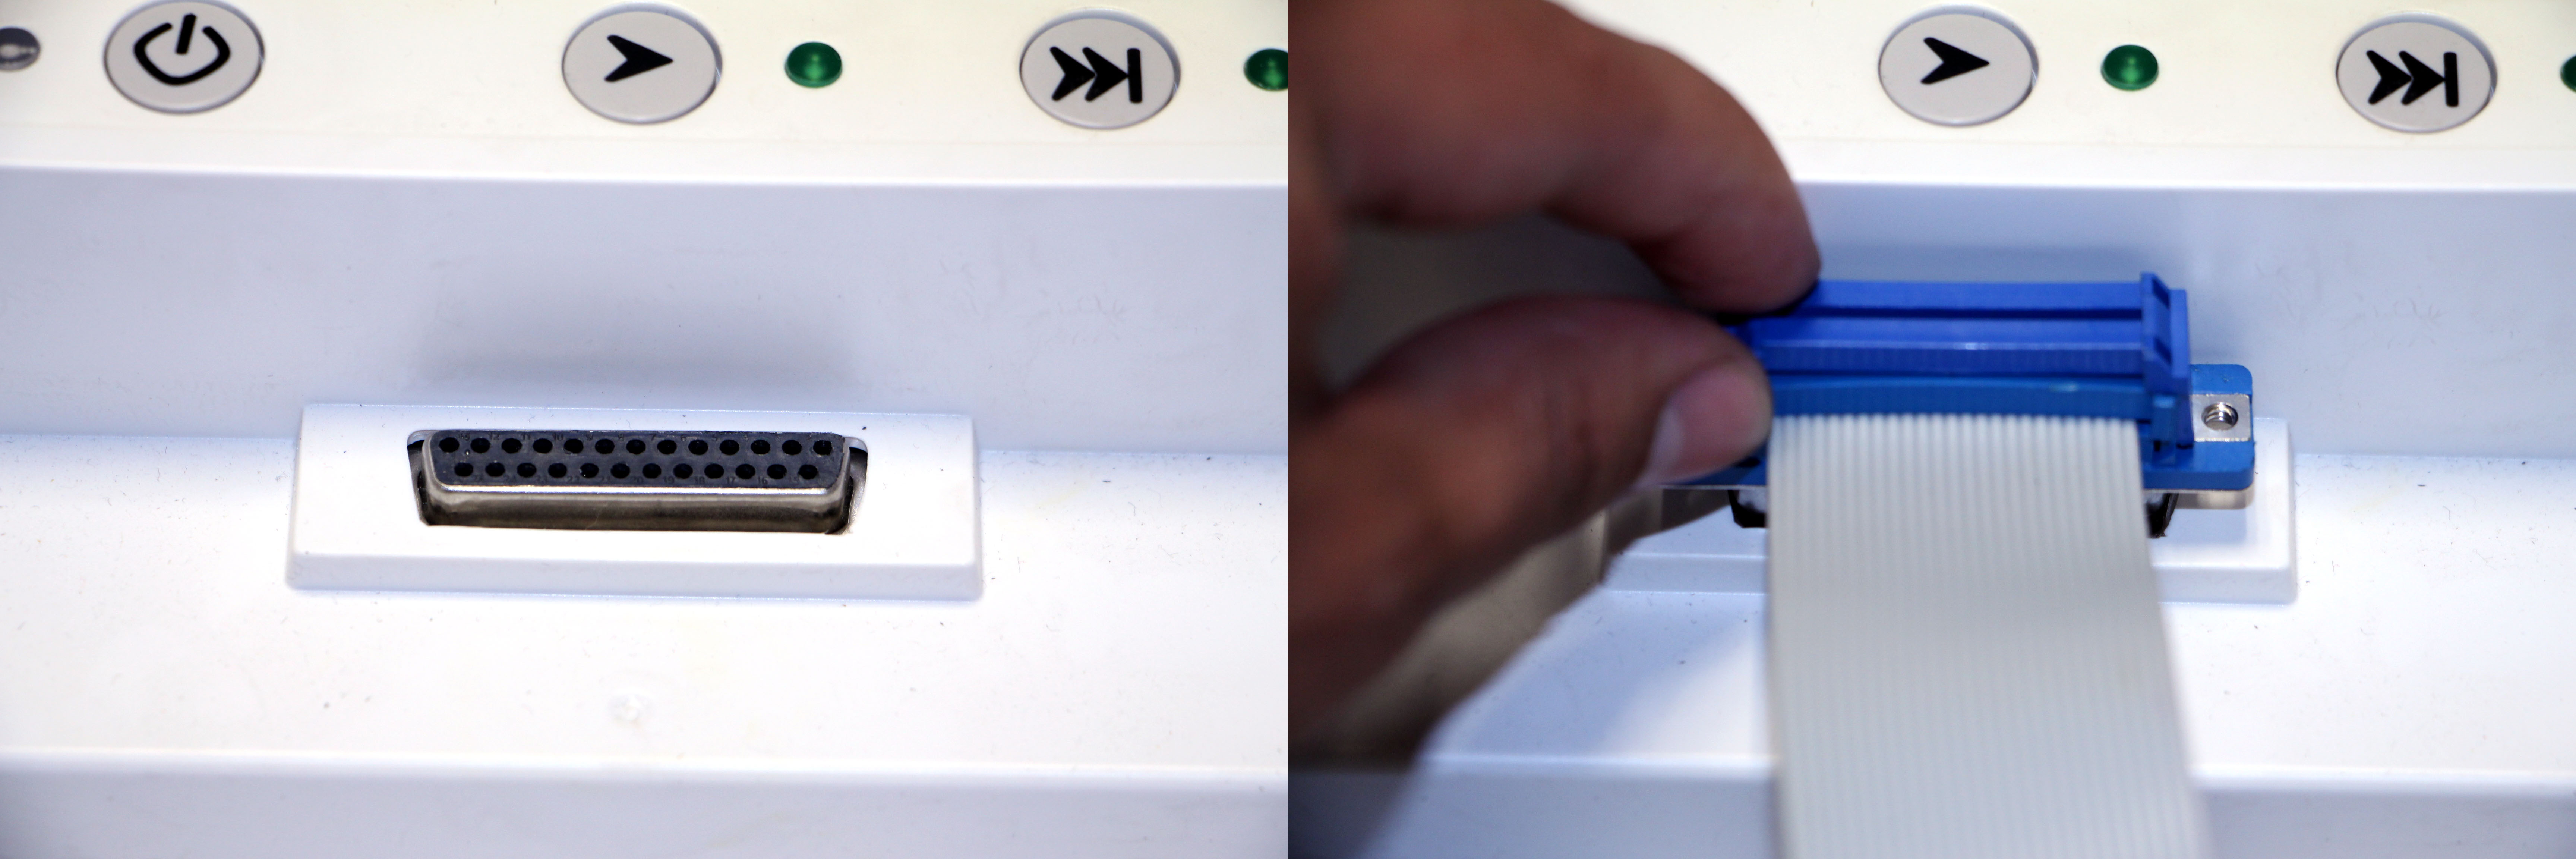
\includegraphics[width=0.8\textwidth]{figures/cargo.jpg}
\caption{Conector DB-25 en la bahía de carga del Create\textsuperscript{\textregistered}}
\centering
\label{fig:cargoCable}
\end{center}
\end{figure} 
2. Conecte un cable USB al puerto puerto correspondiente de la placa fenólica como se muestra en la figura \ref{fig:usbCable}.\\
\begin{figure}
\begin{center}
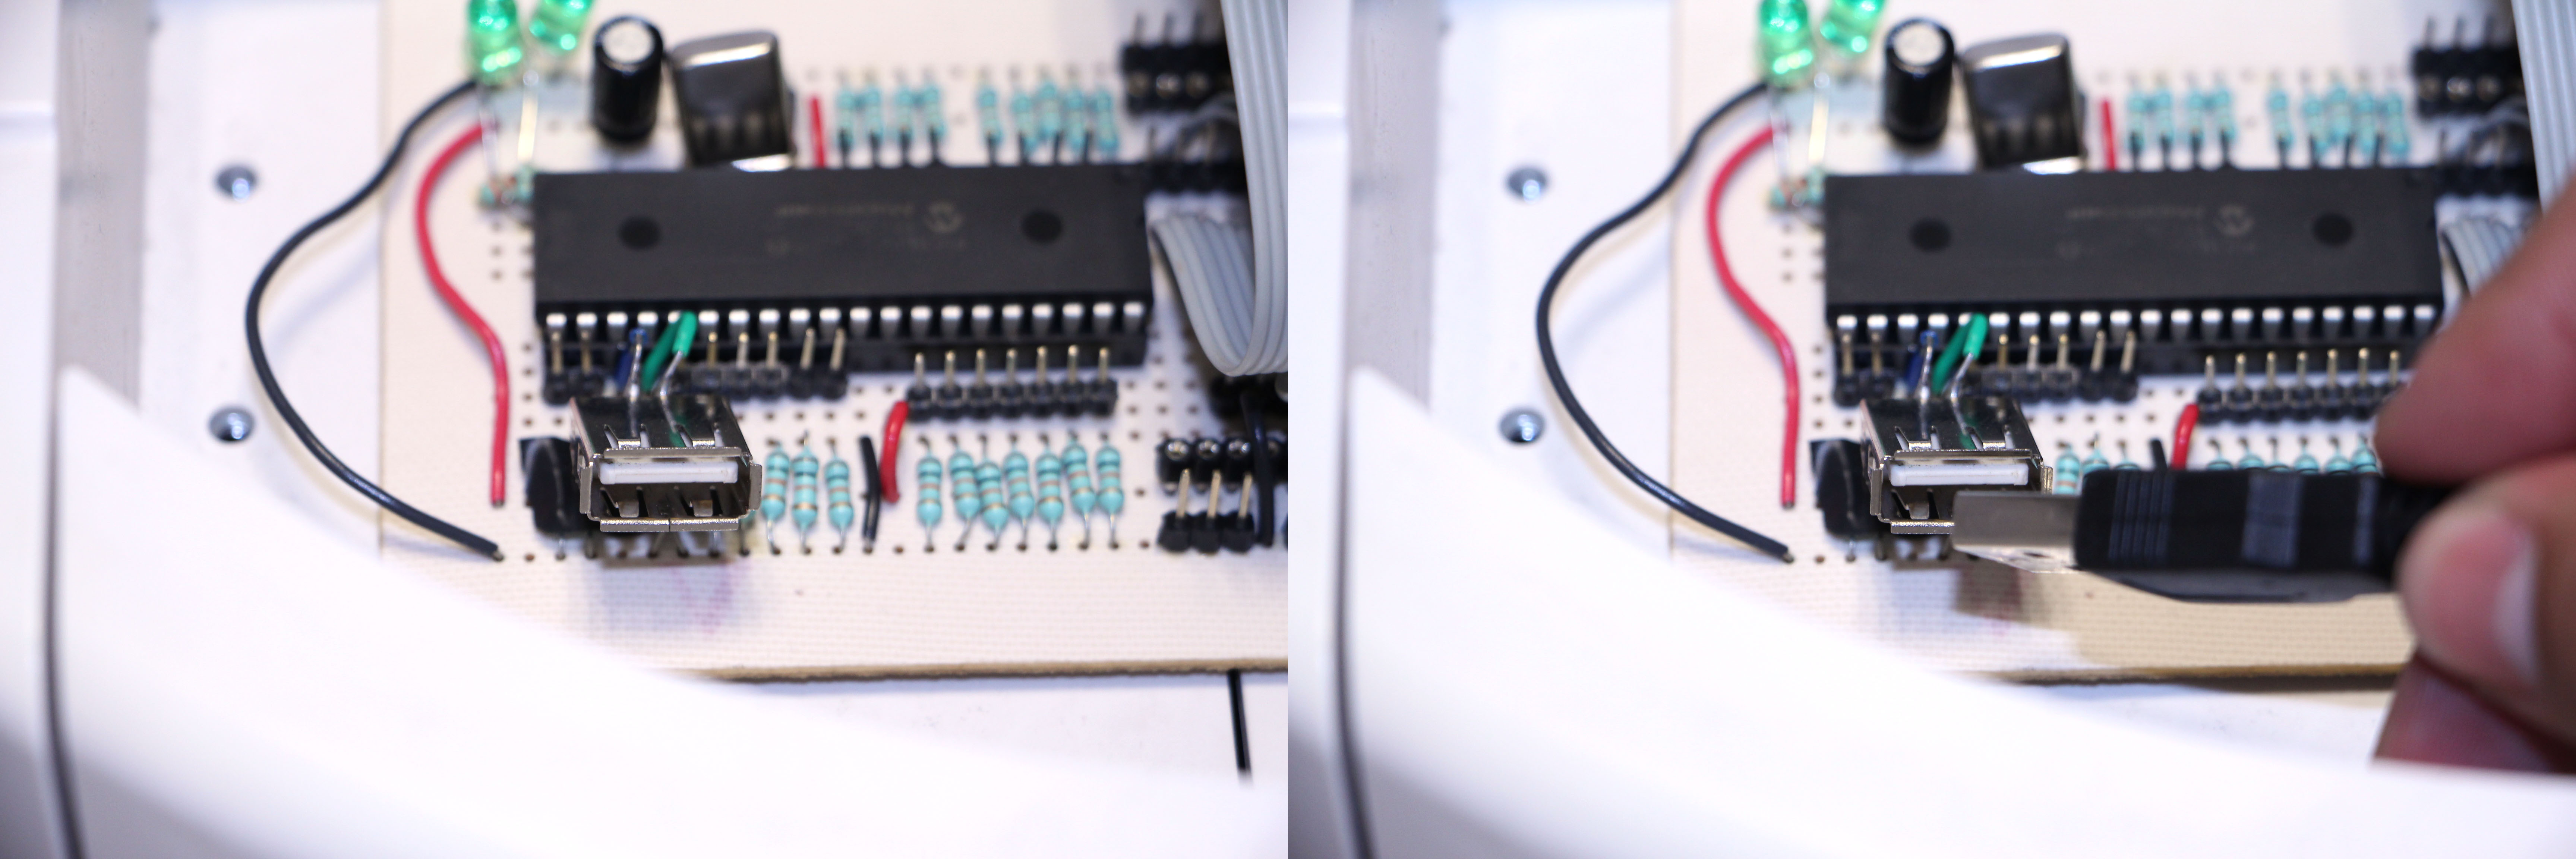
\includegraphics[width=0.8\textwidth]{figures/usbcable.jpg}
\caption{Conexión de los sensores externos mediante un cable USB}
\centering
\label{fig:usbCable}
\end{center}
\end{figure} 
3. Conecte un cable serial al conector DB-9 de la placa fenólica como se ilustra en la figura \ref{fig:serialCable}. Es posible utilizar un convertidor serial/usb si su PC no posee un puerto serial.\\
\begin{figure}
\begin{center}
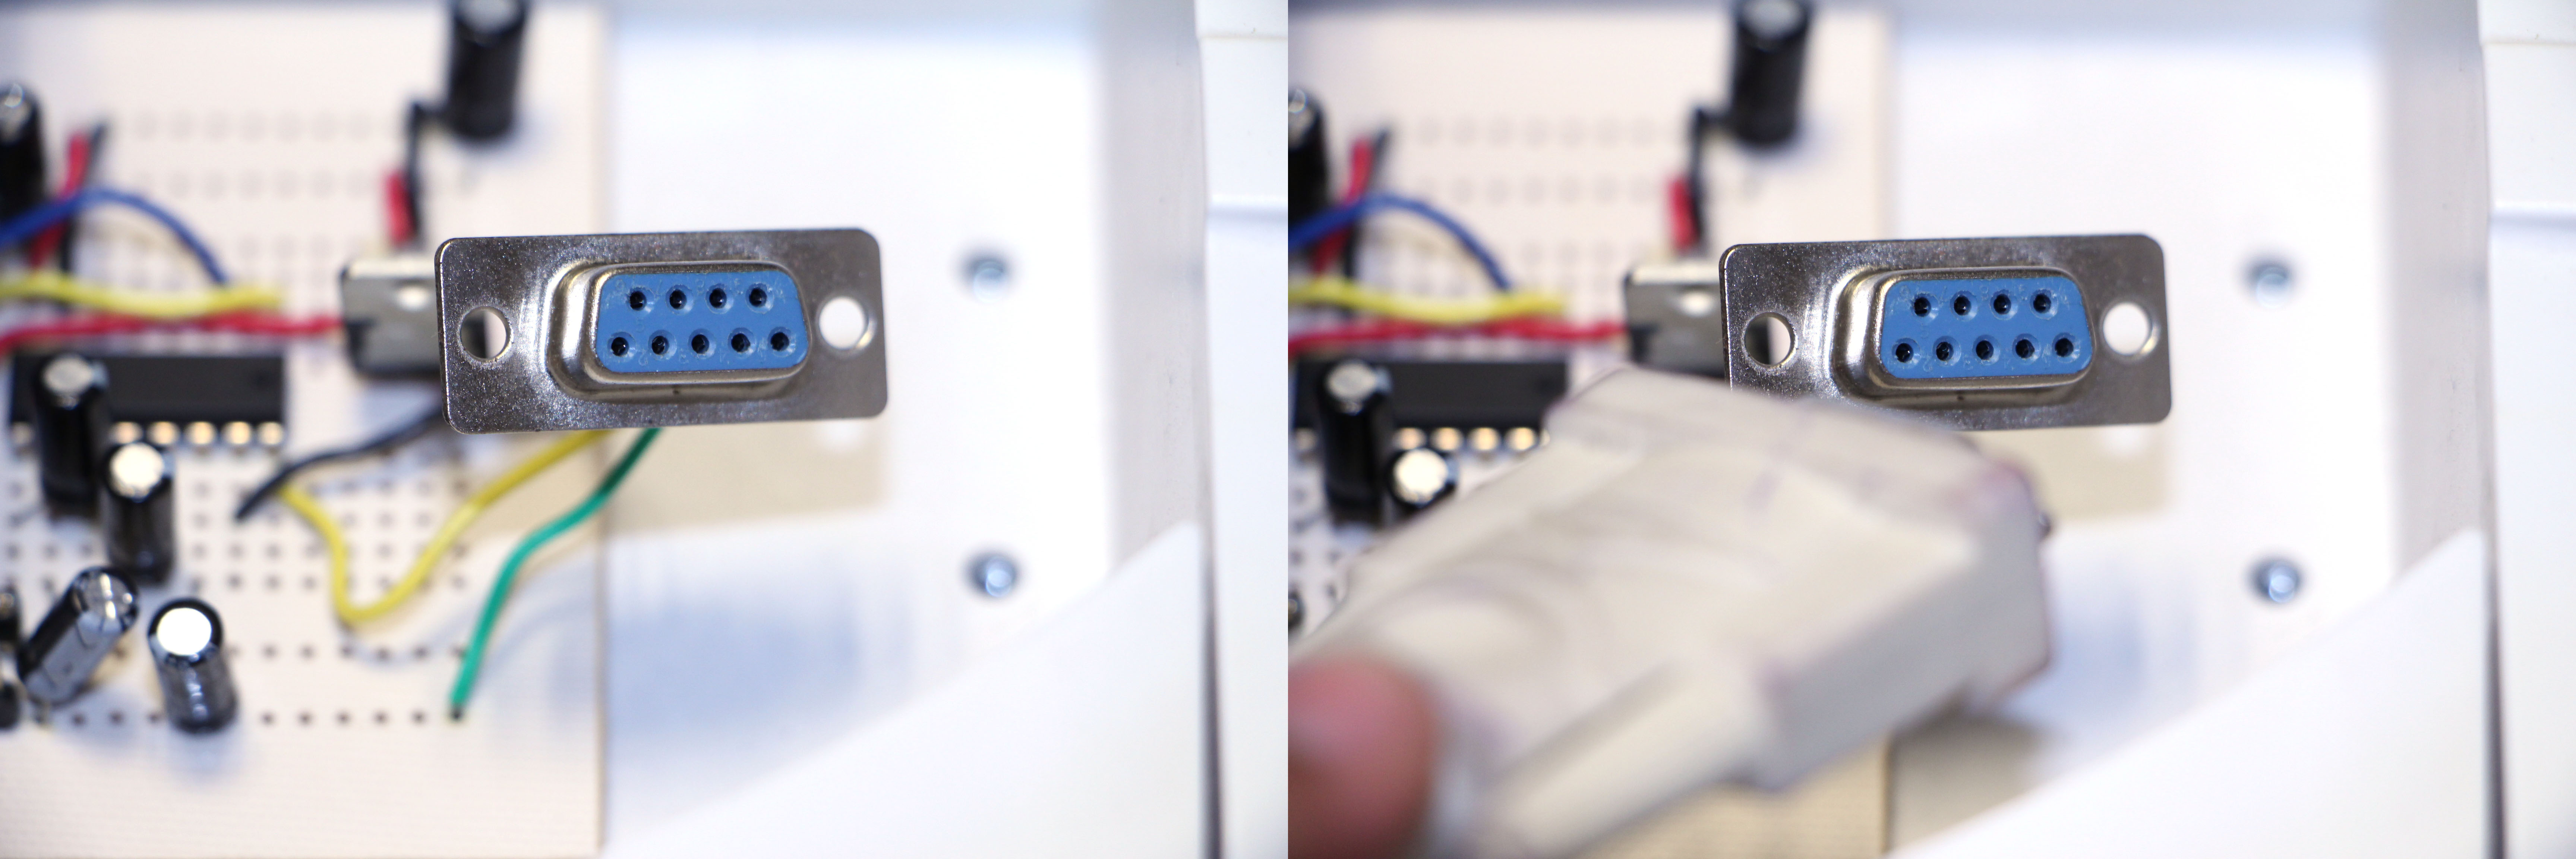
\includegraphics[width=0.8\textwidth]{figures/serialcable.jpg}
\caption{Conector DB-9 para la comunicación serial}
\centering
\label{fig:serialCable}
\end{center}
\end{figure} 
4. Para conectar sensores externos, tanto analógicos como digitales, se recomienda que estos tengan terminales acopladas a las puntas. Por seguridad, la terminal VCC del sensor debe ser macho y el resto hembras (ver figura \ref{fig:cables}). Conecte las terminales de alimentación de los sensores a la placa fenólica. El identificador de sensor en el software será  interpretado de acuerdo a la posición de la conexión física de la terminal de señal. Esto se ilustra en la figura \ref{fig:sensors}.\\
\begin{figure}
\begin{center}
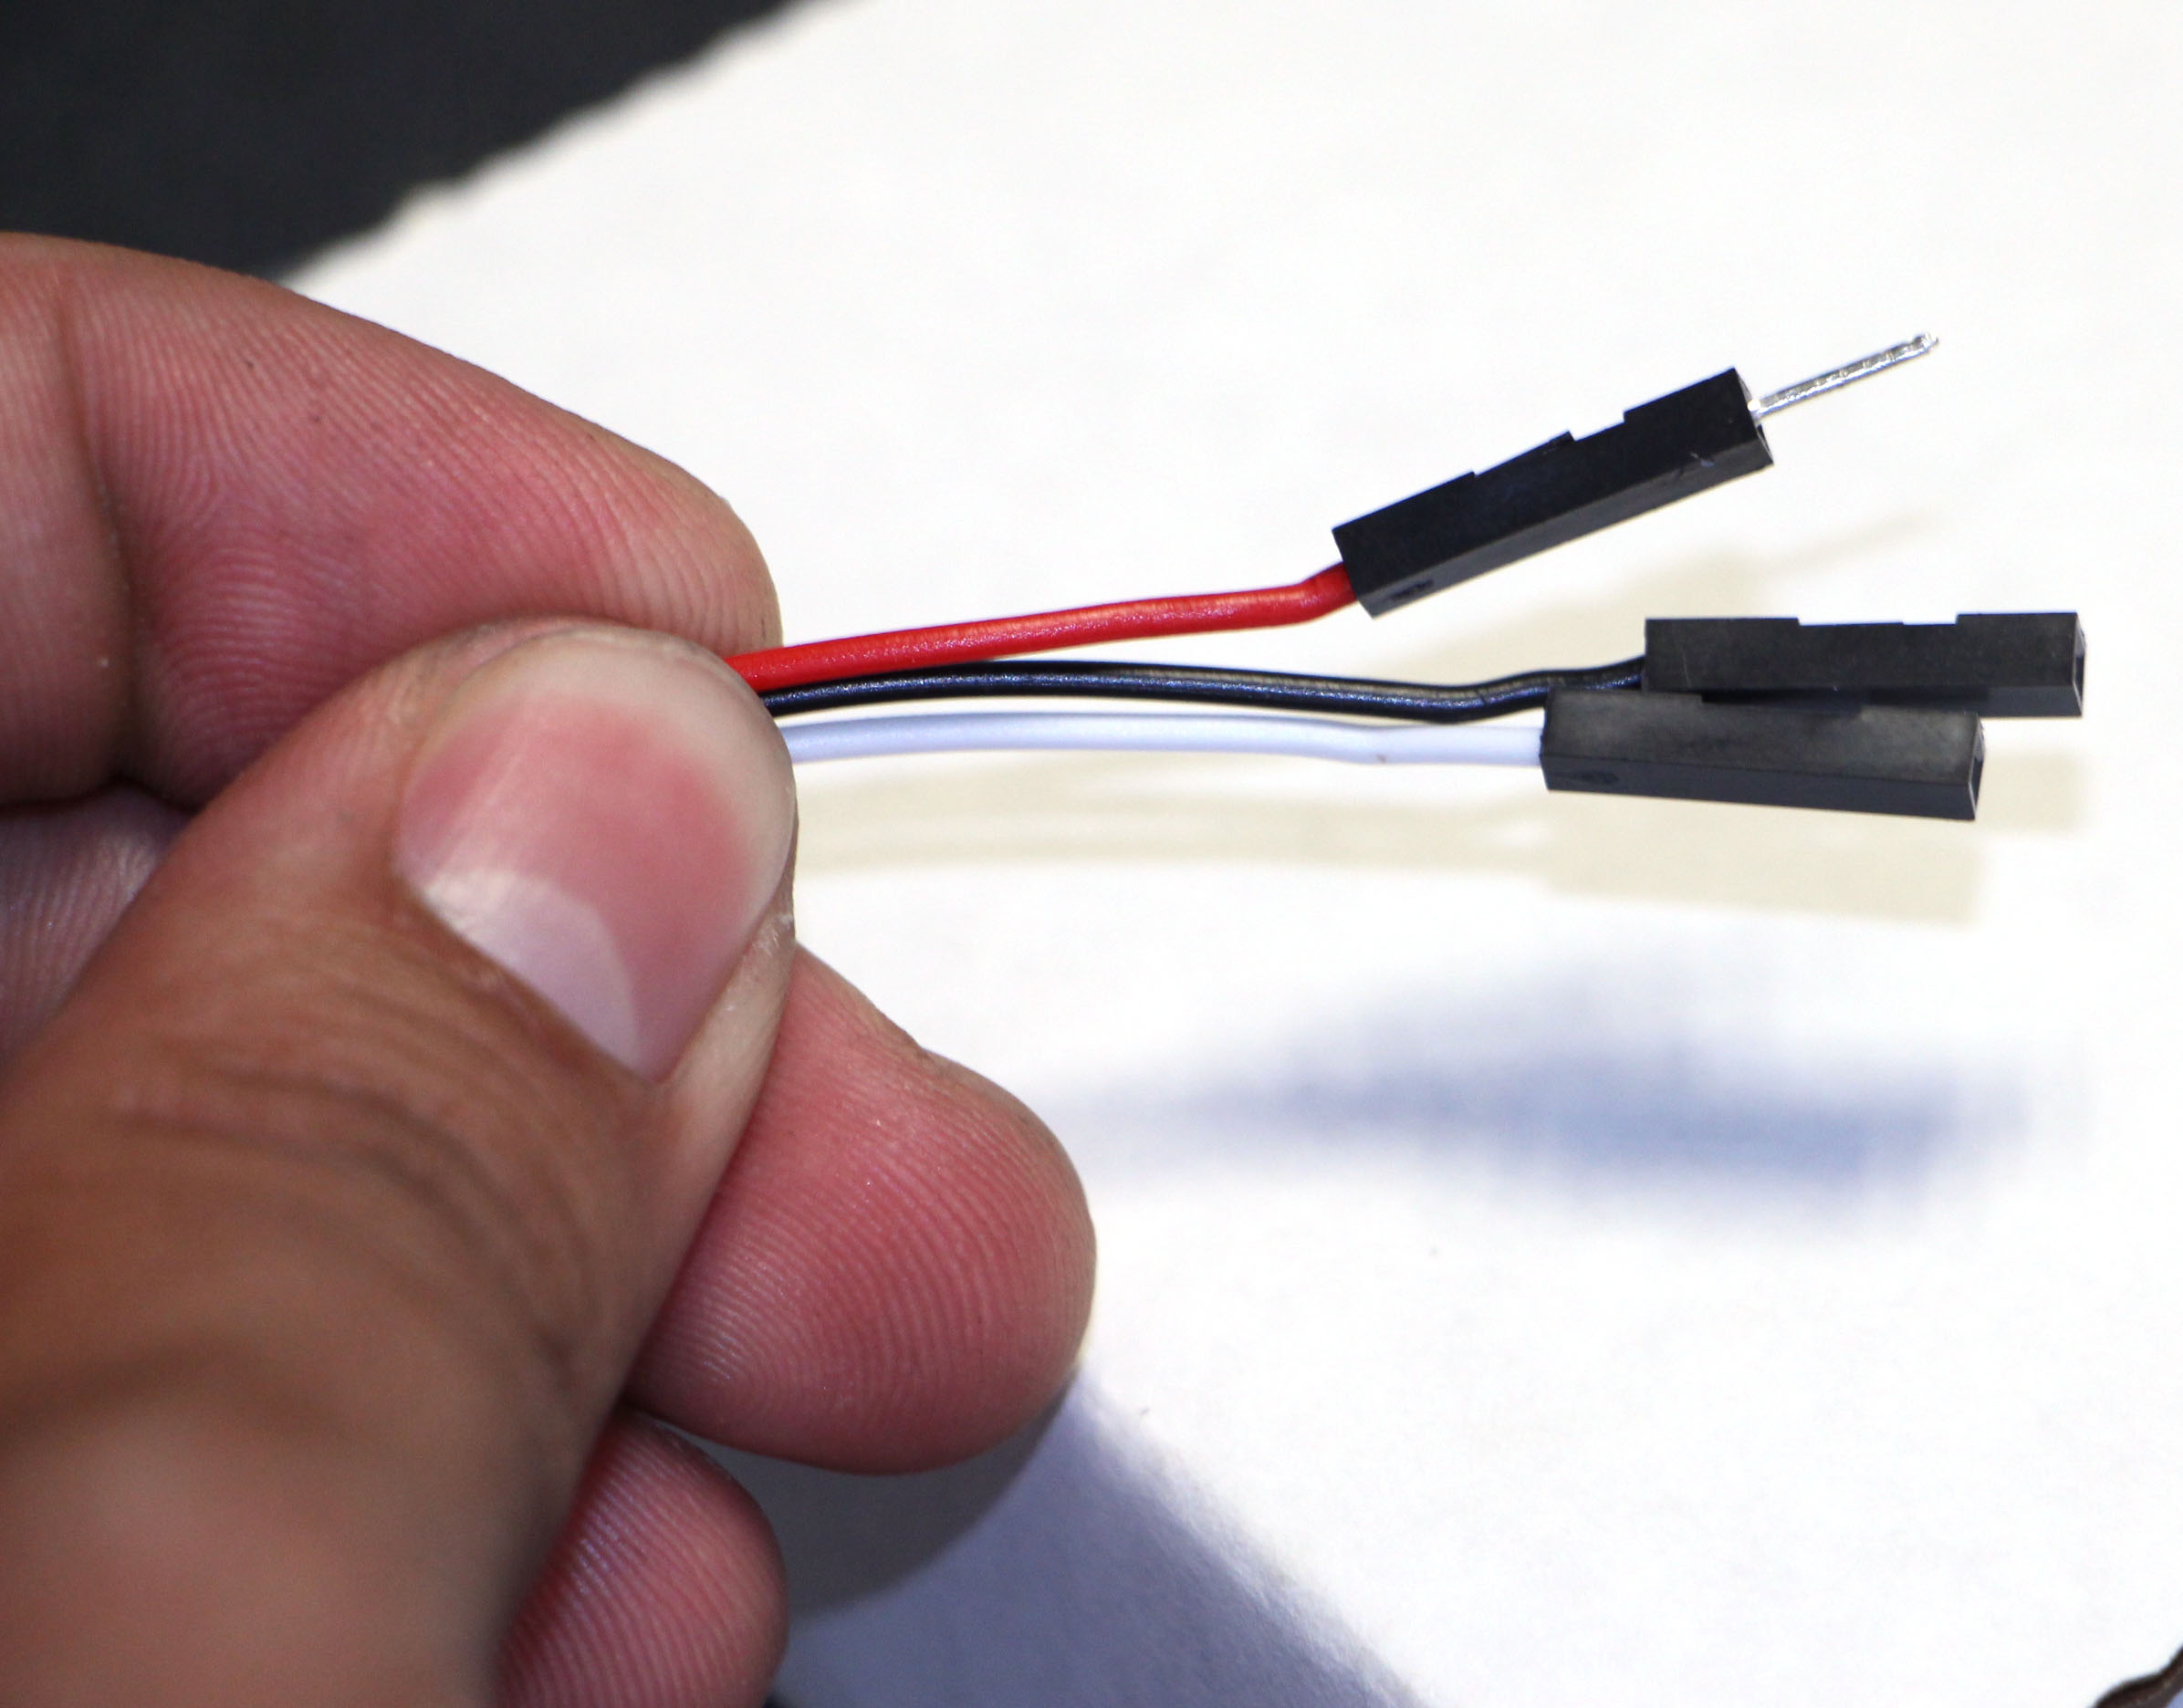
\includegraphics[width=0.8\textwidth]{figures/cables.jpg}
\caption{Terminales para cables recomendadas}
\centering
\label{fig:cables}
\end{center}
\end{figure} 
\begin{figure}
\begin{center}
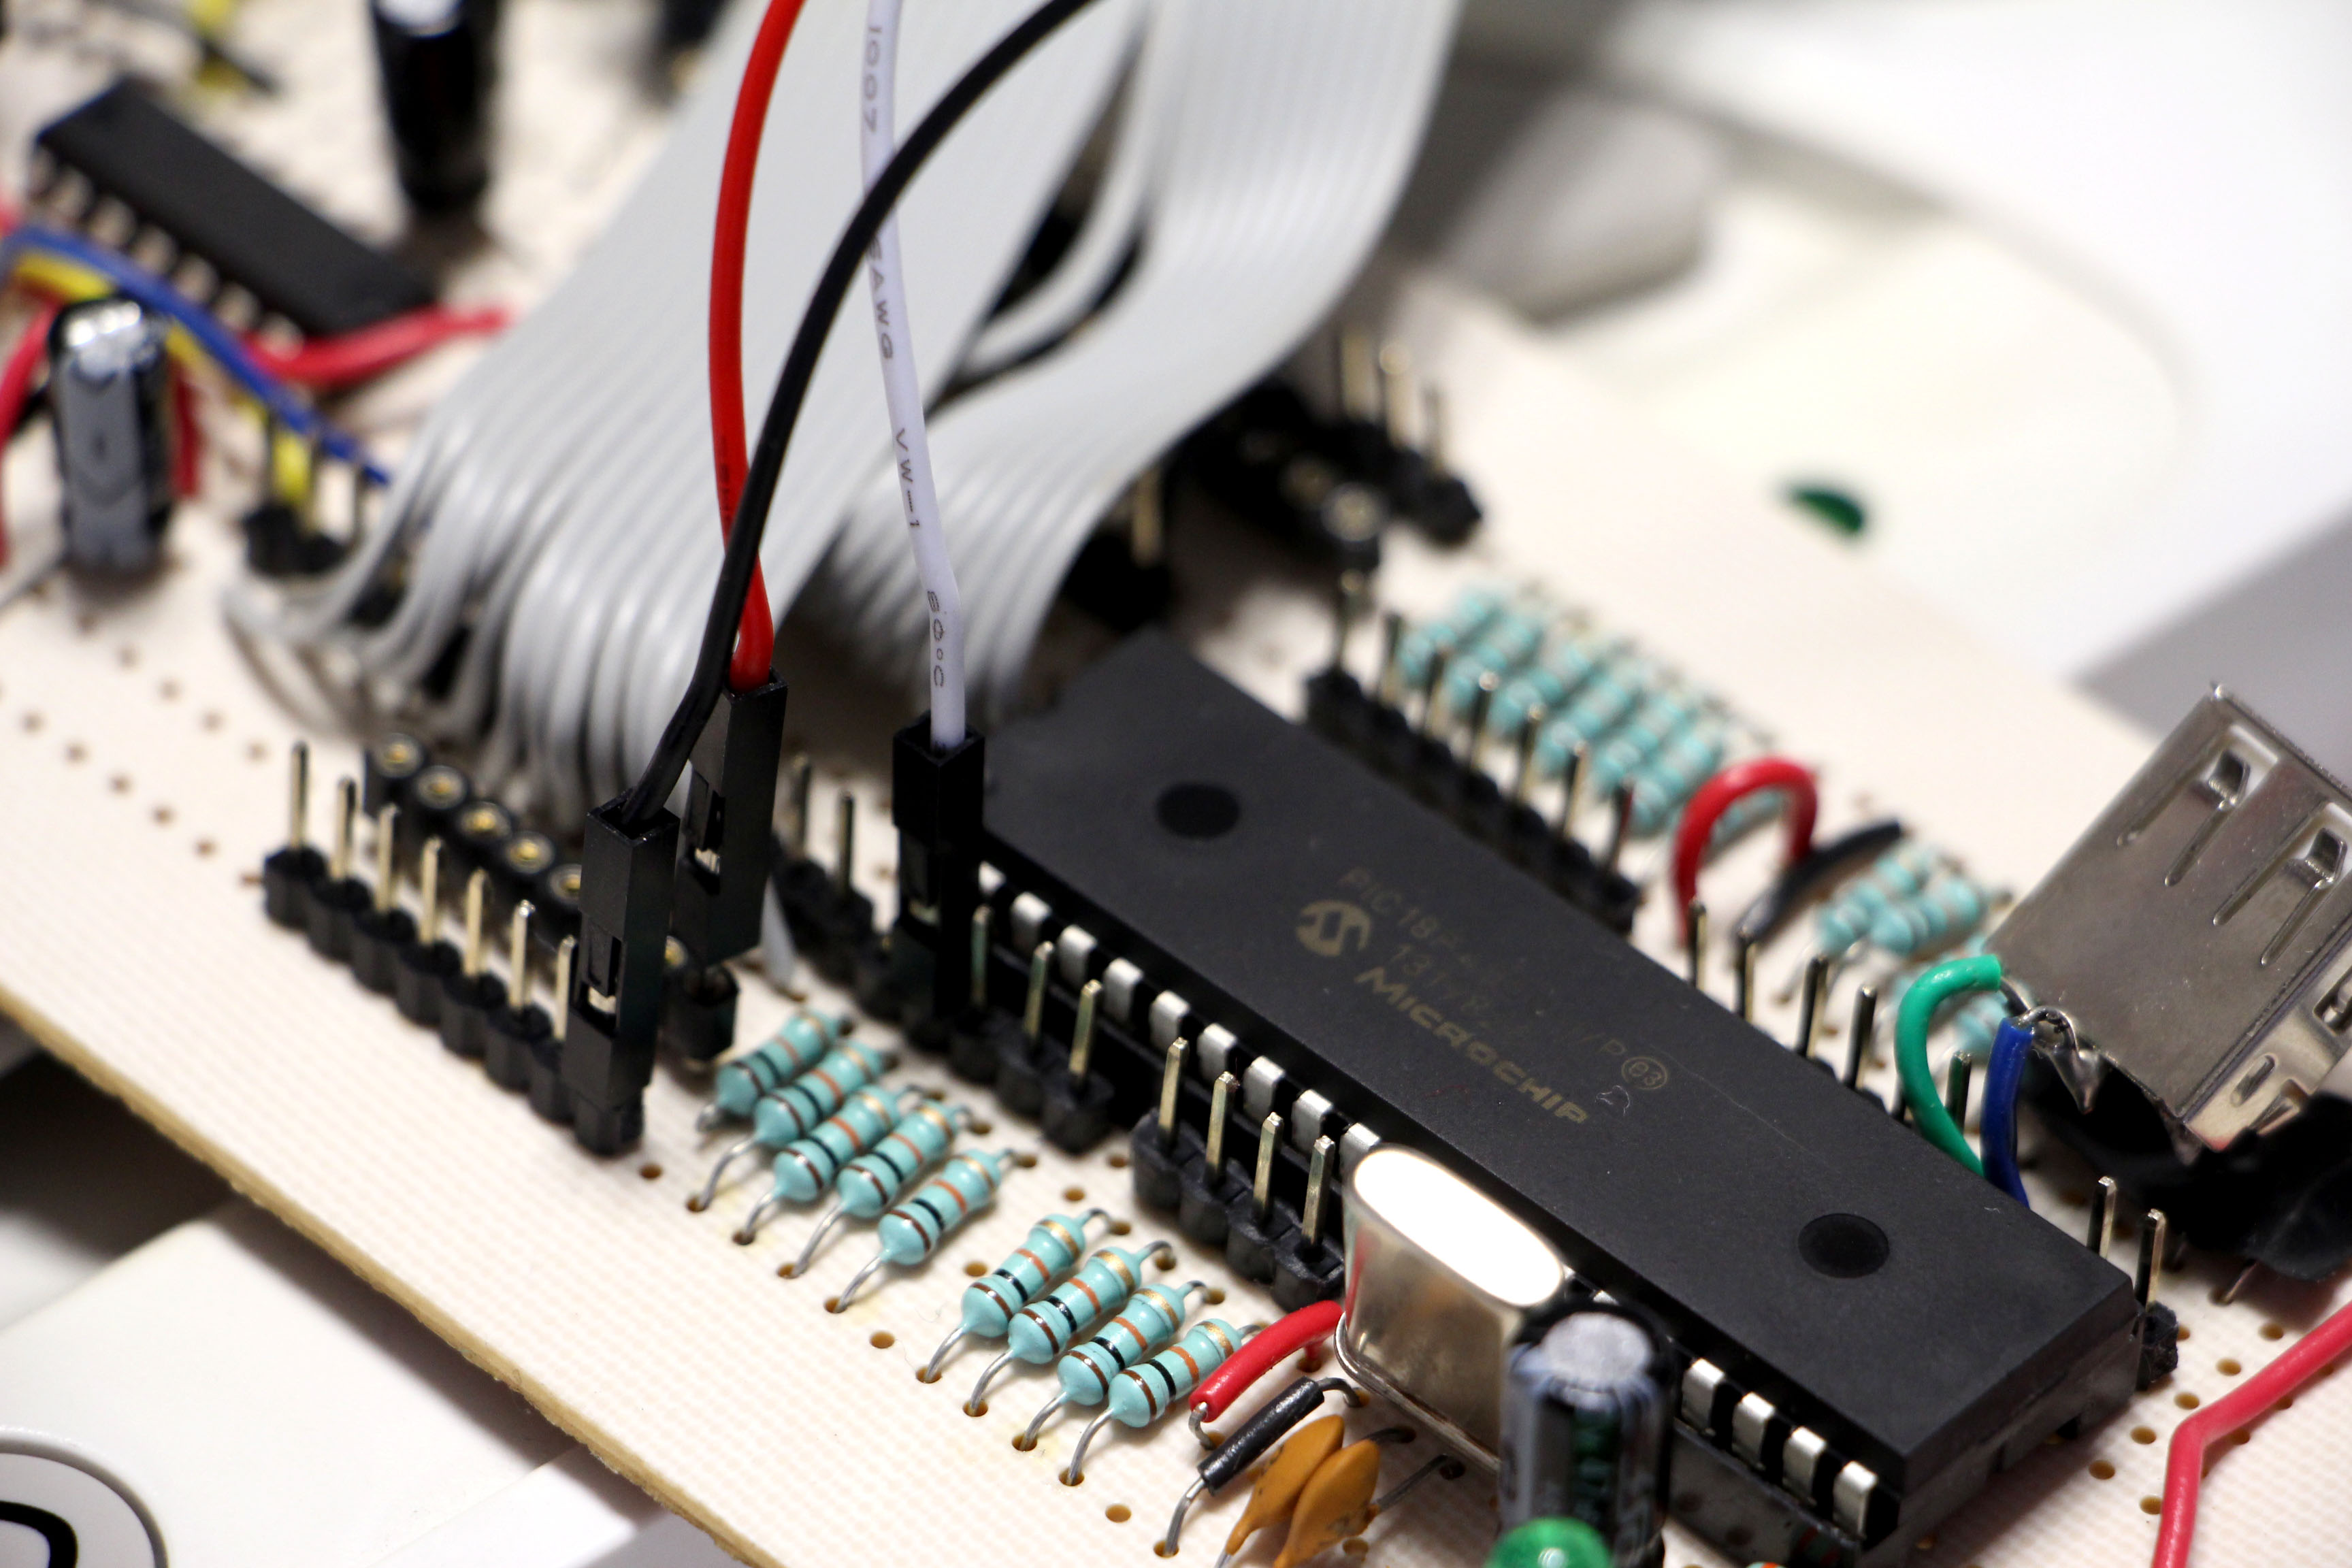
\includegraphics[width=0.8\textwidth]{figures/sensors.jpg}
\caption{Conexión de sensores externos}
\centering
\label{fig:sensors}
\end{center}
\end{figure} 
5. Conecte el otro extremo de los cables serial y USB a la PC (ver figura \ref{fig:computerCables}).\\
\begin{figure}
\begin{center}
\includegraphics[width=0.8\textwidth]{figures/computerCables.jpg}
\caption{Conexión de la placa fenólica a la PC}
\centering
\label{fig:computerCables}
\end{center}
\end{figure} 
6. Una vez realizadas estas conexiones, el robot está listo para usarse. Para aprovechar al máximos las capacidades de la biblioteca UDG\_Create se recomienda utilizar una computadora portátil y montarla junto con los sensores sobre el robot como se muestra en la figura \ref{fig:usage}, sin embargo, otras técnicas como la utilización de hardware intermedio para la comunicación Wi-Fi o Zigbee son también posibles.
\begin{figure}
\begin{center}
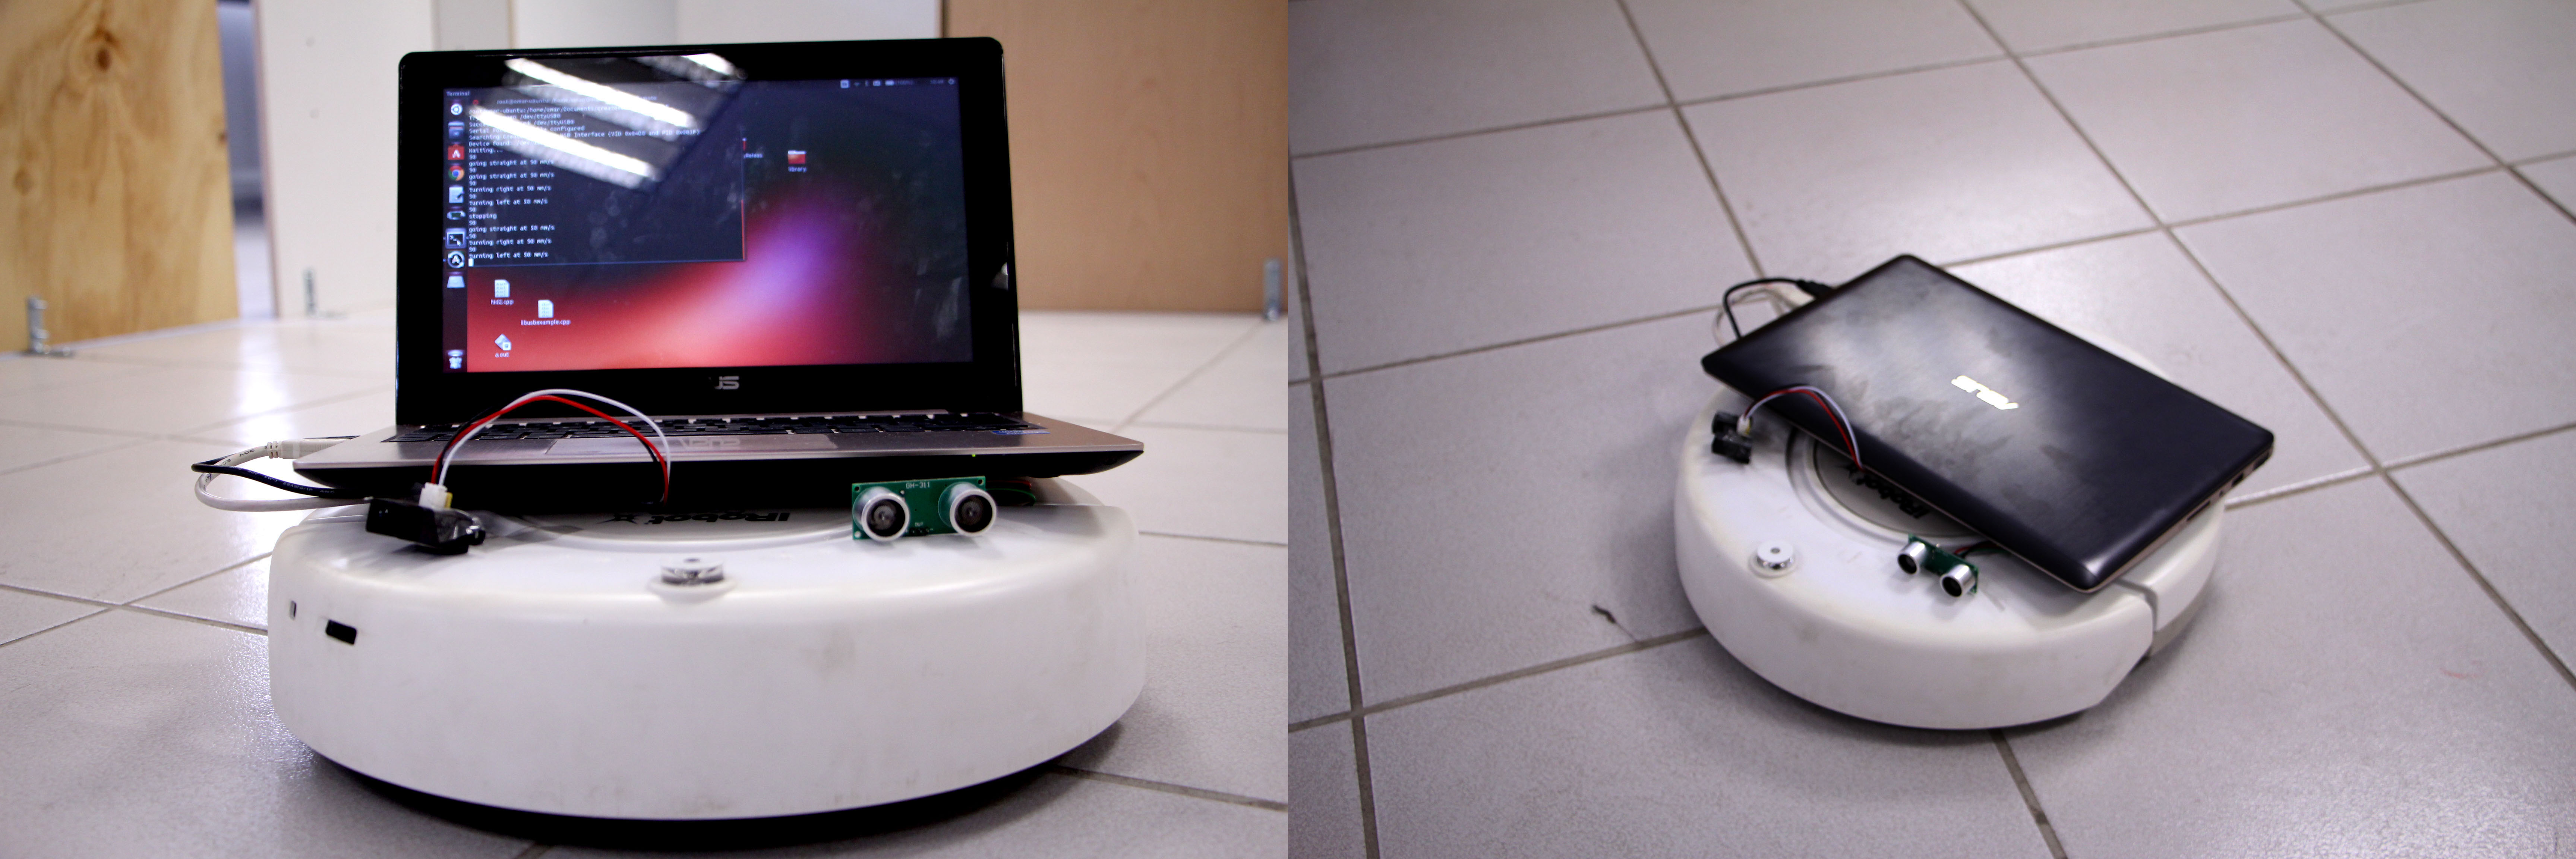
\includegraphics[width=0.8\textwidth]{figures/usage.jpg}
\caption{Modo de uso recomendado}
\centering
\label{fig:usage}
\end{center}
\end{figure}
\section{Dependencias de software}
Para utilizar la biblioteca UDG\_Create es necesario contar con un sistema operativo basado en linux para la arquitectura x86. Durante la ejecución se requieren permisos de root para la lectura de los sensores externos USB. Para recompilar la biblioteca es necesario contar con un compilador que cumpla con el estándar c++ 11. En esta guía de usuario se utilizan Ubuntu 13.10 y g++ 4.7.
\section{Recompilación de la biblioteca con g++}
La biblioteca UDG\_Create se distribuye como una paquete precompilado. Si necesita recompilarla puede hacerlo de manera automática ejecutando el script \emph{rebuildLibrary.sh} contenido en la carpeta del código fuente. Se recomienda utilizar los siguientes comandos:\\
\emph{cd \textless directorio\_del\_codigo\_fuente \textgreater}\\
\emph{sh rebuildLibrary.sh}\\
Para compilaciones personalizadas se requiere llevar a cabo los siguientes pasos:\\
Compilar los archivos fuente (sin ligado).\\
\emph{g++ -c -std=c++11  USBLayer.cpp  ExternalSensors.cpp  UDG\_Create.cpp SerialPort.c }\footnote{Para veriones de g++ 4.3 y posteriores pero inferiores a 4.7 utilizar -std=c++0x en lugar de -std=c++11} \\
Empaquetado del código objeto.\\
\emph{ar rvs UDG\_Create.a ExternalSensors.o  UDG\_Create.o SerialPort.o USBLayer.o}\\
De manera opcional, para utilizar UDG\_Create.h como archivo de encabezado estandar debe agregar el prefijo lib al nombre del paquete.\\
\emph{\emph{ar rvs libUDG\_Create.a ExternalSensors.o  UDG\_Create.o SerialPort.o USBLayer.o}\\}\\
Por último, si asi lo desea, puede eliminar los archivos intermedios generados durante el proceso.\\
\emph{rm *.o}
\section{Uso de UDG\_Create de manera local}
Copie los archivos UDG\_Create.h y UDG\_Create.a al directorio del código fuente de su proyecto.\\
Asegurese de que su programa incluya a la biblioteca como \emph{\#include ``UDG\_Create.h''} (con comillas).\\
Incluya UDG\_Create.a a su comando de compilación para realizar el ligado utilizando la bilioteca. Por ejemplo, para el programa:\\


\begin{lstlisting}[caption={main.cpp}]
#include "UDG_Create.h"
int main()
{
	Create robot;
	robot.demo(9);
	return 0;
}

\end{lstlisting}

Puede utilizar:\\
\emph{g++ main.cpp UDG\_Create.a}

\section{Uso de UDG\_Create como biblioteca estándar}
Copiar UDG\_Create.h a uno de los directorios por defecto para archivos de encabezado (por ejemplo /usr/include/) o usar la opción -I de g++ para especificar la ruta al momento de compilar.\\
Copiar libUDG\_Create.a a uno de los directorios por defecto de c++ para bibliotecas (por ejemplo /usr/lib/) o usar la opción -L de g++ para especificar la ruta en el momento de la compilación.
La biblioteca debe  incluirse en el código fuente como \emph{\#include {\textless}UDG\_Create.h\textgreater} (con paréntesis angulares).\\
Agregue -lUDG\_Create a su comando de compilación para realizar el ligado utilizando la biblioteca. Por ejemplo para el programa\\
\begin{lstlisting}[caption={main.cpp}]
#include <UDG_Create.h>
int main()
{
	Create robot;
	robot.demo(9);
	return 0;
}

\end{lstlisting}

puede usar:
\emph{g++ main.cpp -lUDG\_Create}


\chapter{La Clase Create}
La clase de c++ Create, esta contenida en el archivo UDG\_Create.h y en ella se describe la abstracción de los sensores, actuadores y otros componentes del robot además de todas las operaciones necesarias para la inicialización y operación de los módulos RS-232 y USB.
\section{Tipos de datos y enumeraciones}
\subsection{enum errorCodes}
Define los códigos de error para distintas condiciones de falla durante la ejecución de un programa.\\
INVALID\_DEMO (0x00): El número de modo de desmostración seleccionado no existe.\\
INVALID\_BAUDRATE (0x01): Se ha seleccionado una velocidad de transmisión no válida.\\
INVALID\_INSTRUCTION\_MODE (0x02): Se ha intentado ejecutar una instrucción en un modo que no lo permite.\\
OUT\_OF\_RANGE (0x03): El parámetro seleccionado está fuera del rango permitido.\\
INVALID\_MODE (0x04): Se ha seleccionado un modo de operación inexistente.\\

\subsection{enum modes}
Enlista los distintos modos en los que puede operar el robot.\\
OFF: Robot apagado.\\
PASSIVE: En el modo pasivo es posible ejectutar los programas de demostración asi como leer y escribir información de sensores, pero no se permite ejecutar comandos de actuadores.\\
SAFE: En el modo seguro se tiene control total del robot, pero este regresa a modo pasivo si se detecta un borde (por el que el robot pudiera caer), se solicita un radio de giro menor al radio del robot o se conecta el cargador.\\
FULL: Se tiene control absouluto del robot.\\
\subsection{enum baudCode}
Enumera las velocidades de transmisión soportadas por el Create\textsuperscript{\textregistered}. Las constantes tienen un nombre de la forma BAUDX en donde X representa la velocidad de transmisión en baudios.\\
BAUD300 (0x00).\\
BAUD600 (0x01).\\
BAUD1200 (0x02).\\
BAUD2400 (0x03).\\
BAUD4800 (0x04).\\
BAUD9600 (0x05).\\
BAUD14400 (0x06).\\
BAUD19200 (0x07).\\
BAUD28800 (0x08).\\
BAUD38400 (0x09).\\
BAUD57600 (0x0A).\\
BAUD115200 (0x0B).\\

\subsection{enum  chargingstates}
Describe los posibles estados de carga en los que pudiera encontrarse el robot. La documentación del fabricante no proporciona información adicional respecto a estas condiciones, se asumen autoexplicativas.\\
NOT\_CHARGING (0x00).\\
RECONDITIONING\_CHARGING (0x01).\\
FULL\_CHARGING (0x02).\\
TRICKLE\_CHARGING (0x03).\\
WAITING (0x04).\\
CHARGING\_FAULT\_CONDITION (0x05).\\

\subsection{enum infraredbytechars}
Define los posibles valores que pudieran recibirse a través del receptor infrarrojo provenientes del control remoto, la base de carga, otros robots o aplicaciones externas. La documentación del fabricante no proporciona información adicional por lo que los valores se asumen autoexplicativos.\\
IRLEFT (0x81).\\
IRFORWARD (0x82).\\
IRRIGHT (0x83).\\
IRSPOT (0x84).\\
IRMAX (0x85).\\
IRSMALL (0x86).\\
IRMEDIUM (0x87).\\
IRLARGE (0x88).\\
IRPAUSE (0x89).\\
IRPOWER (0x8A).\\
IRARC\_FORWARD\_LEFT (0x8B).\\
IRARC\_FORWARD\_RIGHT (0x8C).\\
IRDRIVE\_STOP (0x8D).\\
IRSENDALL (0x8E).\\
IRSEEKDOCK (0x8F).\\
IRRESERVED (0x90).\\
IRRED (0x91).\\
IRGREEN (0x92).\\
IRFORCEFIELD (0x93).\\
IRREDGREEN (0x94).\\
IRREDFORCEFIELD (0x95).\\
IRGREENFORCEFIELD (0x96).\\
IRREDGREENFORCEFIELD (0x97).\\

\subsection{enum sensorPackets}
Define los el numero asociado a cada paquete de los disponibles como argumento de la funcion GetSensors().\\
S\_PACKET0(0x00)\\
S\_PACKET1(0x01)\\
S\_PACKET2(0x02)\\
S\_PACKET3(0x03)\\
S\_PACKET4(0x04)\\
S\_PACKET5(0x05)\\
S\_PACKET6(0x06)\\
S\_BUMPS\_AND\_WHEEL\_DROPS(0x07)\\
S\_WALL(0x08)\\
S\_CLIFF\_LEFT(0x09)\\
S\_CLIFF\_FRONT\_LEFT(0x0A)\\
S\_CLIFF\_FRONT\_RIGHT(0x0B)\\
S\_CLIFF\_RIGHT(0x0C)\\
S\_VIRTUAL\_WALL(0x0D)\\
S\_OVERCURRENTS(0x0E)\\
S\_UNUSED1(0x0F)\\
S\_UNUSED2(0x10)\\
S\_IR\_BYTE(0x11)\\
S\_BUTTONS(0x12)\\
S\_DISTANCE(0x13)\\
S\_ANGLE(0x14)\\
S\_CHARGING\_STATE(0x15)\\
S\_VOLTAGE(0x16)\\
S\_CURRENT(0x17)\\
S\_BATTERY\_TEMPREATURE(0x18)\\
S\_BATTERY\_CHARGE(0x19)\\
S\_BATTERY\_CAPACITY(0x1A)

\subsection{ enum VerbosityLevels}
VERBOSITY\_NORMAL (0x00): Los mensajes del robot se escriben a la salida estándar.\\
VERBOSITY\_FILE (0x01): Los mensajes del robot se escriben a un archivo.\\
VERBOSITY\_OFF (0x02): No se escribe ningun mensaje.\\
VERBOSITY\_NUMBER\_OF\_LEVELS (0x03): El número total de niveles.\\

\subsection{t\_verbosity}
Tipo de dato enumerado que corresponde a los valores de VerbosityLevels.\\

\subsection { enum BoolSigned}
SIGNED (0x01).\\
UNSIGNED (0x02).\\
\subsection{ boolSigned}
Tipo de dato enumerado que corresponde a los valores de BoolSigned y se utiliza para indicar si los elementos en un arreglo de bytes debe ser considerado como un número con o sin signo.\\

\subsection{ NUMBER\_OF\_SENSORS }
Describe el máximo número de sensores externos que pueden conectarse a la interfaz USB.\\

\subsection{int16}
Entero de 16 bits, utilizado para garantizar su tamaño idependientemente del compilador. Su definición exacta es:\\
\begin{lstlisting}
typedef struct int_16
{
	unsigned char H; //High byte
	unsigned char L; //Low byte
} int16;
\end{lstlisting}

\section{Miembros (privados)}
\subsection{std::string portName}\mbox{}\\
Una cadena que indica el nombre del enlace simbólico asociado a la comunicación serial con el robot.
\subsection{int mode}\mbox{}\\
Un valor definido en la enumeración \emph{oimodes} que indica el modo de operación actual del robot.
\subsection{bool charging}\mbox{}\\
Una variable lógica que indica si el robot está siendo cargado.
\subsection{int portDescriptor}\mbox{}\\
El descriptor del puerto asociado a la comunicación serial con el robot.
\subsection{int baudRate}\mbox{}\\
Un valor perteneciente a la enumeración \emph{baudCode} que indica la velocidad de transmisión utilizada para la comunicación serial.
\subsection{bool bumpRight}\mbox{}\\
Una variable lógica que indica si el lado derecho del parachoques está siendo presionado.
\subsection{bool bumpLeft}\mbox{}\\
Una variable lógica que indica si el lado izquierdo del parachoques está siendo presionado.
\subsection{bool wheelDropRight}\mbox{}\\
Una variable lógica que indica si el sensor de caída de la rueda derecha fué activado.
\subsection{bool wheelDropLeft}\mbox{}\\
Una variable lógica que indica si el sensor de caída de la rueda izquierda fué activado.
\subsection{bool wheelDropCaster}\mbox{}\\
Una variable lógica que indica si el sensor de caída de la rueda caster fué activado.
\subsection{bool wall}\mbox{}\\
Una variable lógica que indica si una pared ha sido detectada.
\subsection{bool cliffLeft}\mbox{}\\
Una variable lógica que indica si un borde ha sido detectado del lado izquierdo.
\subsection{bool cliffFrontLeft}\mbox{}\\
Una variable lógica que indica si el sensor de bordes frontal izquierdo ha sido activado.
\subsection{bool cliffFrontRight}\mbox{}\\
Una variable lógica que indica si el sensor de bordes frontal derecho ha sido activado.
\subsection{bool cliffRight}\mbox{}\\
Una variable lógica que indica si un borde ha sido detectado del lado derecho.
\subsection{bool virtualWall}\mbox{}\\
Una variable lógica que indica si una pared virtual ha sido detectada.
\subsection{bool ld0}\mbox{}\\
Una variable lógica que indica si el \emph{low side driver } 0 está encendido.
\subsection{bool ld1}\mbox{}\\
Una variable lógica que indica si el \emph{low side driver } 1 está encendido.
\subsection{bool ld2}\mbox{}\\
Una variable lógica que indica si el \emph{low side driver } 2 está encendido.
\subsection{bool rightWheel}\mbox{}\\
Una variable lógica que indica si el sensor de sobrecorriente de la rueda derecha ha sido activado.
\subsection{bool leftWheel}\mbox{}\\
Una variable lógica que indica si el sensor de sobrecorriente de la rueda izquierda ha sido activado.
\subsection{unsigned char infraredbyte}\mbox{}\\
Una variable de un byte que almacena la información leída a través del receptor infrarrojo.
\subsection{bool advancebtn}\mbox{}\\
Una variable lógica que indica si el botón \emph{advance} del robot está siendo presionado.
\subsection{bool playbtn}\mbox{}\\
Una variable lógica que indica si el botón \emph{play} del robot está siendo presionado.
\subsection{int distance}\mbox{}\\
Una variable entera que indica la distancia recorrida desde la última vez que se consultó.
\subsection{int angle}\mbox{}\\
Una variable entera que indica el ángulo rotado desde la última vez que se consultó.
\subsection{unsigned char chargingstate}\mbox{}\\
Un miembro de la enumeración \emph{chargingstates} que describe las condiciones actuales de la carga de la batería.
\subsection{int voltage}\mbox{}\\
Una variable entera que representa el voltaje en mV en la batería del robot.
\subsection{int current}\mbox{}\\
La corriente en mA que entra (valores positivos) o sale (valores negativos) de la batería del robot. 
\subsection{unsigned char batterytemperature}\mbox{}\\
La temperatura de la batería del robot en grados celsius.
\paragraph{int batterycharge}\mbox{}\\
La carga de la batería del robot en mAh.
\subsection{int batterycapacity}\mbox{}\\
La capacidad aproximada de la batería en mAh.
\paragraph{int wallsignal}\mbox{}\\
Una variable entera que representa la magnitud de la lectura en el sensor de paredes.
\subsection{int cliffls}\mbox{}\\
Una variable entera que representa la magnitud de la lectura en el sensor de bordes  izquierdo.
\subsection{int clifffls}\mbox{}\\
Una variable entera que representa la intensidad de la lectura en el sensor de bordes frontal izquierdo.
\subsection{int clifffrs}\mbox{}\\
Una variable entera que representa la intensidad de la lectura en el sensor de bordes frontal derecho.
\subsection{int cliffrs}\mbox{}\\
Una variable entera que representa la intensidad de la lectura en el sensor de bordes derecho.
\subsection{bool digitalinput0}\mbox{}\\
Una variable lógica que indica si existe un nivel de voltaje alto en la entrada digital 0.
\subsection{bool digitalinput1}\mbox{}\\
Una variable lógica que indica si existe un nivel de voltaje alto en la entrada digital 1.
\subsection{bool digitalinput2}\mbox{}\\
Una variable lógica que indica si existe un nivel de voltaje alto en la entrada digital 2.
\subsection{bool digitalinput3}\mbox{}\\
Una variable lógica que indica si existe un nivel de voltaje alto en la entrada digital 3.
\subsection{bool baudchangerate}\mbox{}\\
Una variable lógica que indica si hay un nivel de voltaje alto en la terminal correspondiente al cambio de velocidad de transmsión (terminal 15).
\subsection{int cargoanalogsignal}\mbox{}\\
Una variable entera que representa el valor de la señal analógica en la terminal 4 del robot.
\subsection{bool homebase}\mbox{}\\
Una variable lógica que indica si existe una conexión entre el robot y la base de carga.
\subsection{bool internalcharger}\mbox{}\\
Una variable lógica que indica si el cargador interno está conectado.
\subsection{unsigned char oimode}\mbox{}\\
Representa el modo de operación actual del robot como un miembro de la enumeracion \emph{oimodes}.
\subsection{unsigned char songnumber}\mbox{}\\
Indica el número de la canción actualmente seleccionada.
\subsection{bool songplaying}\mbox{}\\
Indica si hay una canción siendo tocada actualmente.
\subsection{unsigned char streampackets}\mbox{}\\
El número de sensores o paquetes de sensores solicitados como parte de un flujo.
\subsection{int reqvelocity}\mbox{}\\
La velocidad de las ruedas solicitada en la última llamada a una instrucción \emph{drive}.
\subsection{int reqradius}\mbox{}\\
El radio de giro solicitado en la última llamada a una función \emph{drive}.
\subsection{int reqrvelocity}\mbox{}\\
La velocidad de la rueda derecha solicitada en la última llamada a una función \emph{drive}.
\subsection{int reqlvelocity}\mbox{}\\
La velocidad de la rueda izquierda solicitada en la última llamada a una función \emph{drive}.
\subsection{bool streamingState}\mbox{}\\
Una variable lógica que indica si un flujo de paquetes de sensores se está transmitiendo actualmente.
\subsection{bool externalSensorsEnabled}\mbox{}\\
Una variable lógica que inidica si los sensores externos conectados por usb están actualmente habilitados.
\subsection{t\_verbosity robotVerbosity}\mbox{}\\
Indica el tipo de mensajes de depuración que se mostrarán en pantalla.


\section{Funciones}
\subsection{Publicas}
\subsubsection{Create()}
Es el método constructor por defecto, inicializa el puerto serial utilizando los primeros enlaces símbolicos para puerto serial y USB disponibles.

\subsubsection{Create( std::string \_portName, t\_verbosity verbosityLevel )}\mbox{}\\
\emph{\_portName: }El nombre del enlace símbolico a utilizar para la comunicación serial.\\
\emph{verbosityLevel: } El tipo de mensajes de depuración a recibir durante la ejecución. Los valores disponibles para este parametro son\\
VERBOSITY\_NORMAL: Los mensajes se imprimen a la salida estándar.\\
VERBOSITY\_OFF: No se imprimen mensajes.\\

\subsubsection{\char126Create()}\mbox{}\\
Es el método destructor por defecto, libera todos los recursos solicitados durante la ejecución.\\

\subsubsection{std::string getPortName()}\mbox{}\\
Regresa un valor de tipo std::string conteniendo el nombre del enlace simbólico utilizado para la inicialización del puerto serial.

\subsubsection{void start()}\mbox{}\\
Prepara al robot para recibir instrucciones por el puerto serial y lo pone en modo pasivo (\emph{passive}).\\

\subsubsection{void baud(unsigned char baudRate)}\mbox{}\\
\emph{baudRate: } La nueva velocidad de transmisión de acuerdo a los valores establecidos en la Create Open Interface.\\\\
Modifica por software la velocidad de transimisión (baud rate) utilizado para la comunicación serial.  Se recomienda utilizar los miembros de la enumeración baudRate de la forma BAUDx en donde x representa la velocidad.\\

\subsubsection{void control()}\mbox{}\\
Pone al robot en modo seguro (safe). Esta función se conserva para mantener compatibilidad con Roomba, se recomienda el uso de la función safe() en su lugar para el Create\textsuperscript{\textregistered}.\\
		
\subsubsection{void safe()}\mbox{}\\
Pone al robot en modo seguro (safe).\\

\subsubsection{void full()}\mbox{}\\
Pone al robot en modo íntegro (full).\\

\subsubsection{void spot()}\mbox{}\\
Ejecuta la demostración ``spot demo'' en la que el robot se mueve formando una espiral. Al terminar de ejecutar la instrucción el Create\textsuperscript{\textregistered} pasa a modo pasivo (passive).\\

\subsubsection{void cover()}\mbox{}\\
Ejecuta la demostración ``cover'' de la Create Open Interface en el que se cubre el área de una habitación.\\

\subsubsection{void coverAndDock()}\mbox{}\\
Ejecuta la demostración ``cover and dock'' de la Create Open Interface.

\subsubsection{void demo( unsigned char demo )}\mbox{}\\
\emph{demo: } El número de la demostración a ejecutar.\\\\
Ejecuta la demostración indicada por \emph{demo}. El número de demo debe estar entre 1 y 9.\\
\subsubsection{void drive( int velocity, int radius )}\mbox{}\\
\emph{speed: } La velocidad promedio a la que girarán las ruedas del robot en mm/s.\\
\emph{radius: }Radio en milimetros del giro del robot medido desde el centro del circulo de giro hasta el centro del Create\textsuperscript{\textregistered}.\\\\

Controla las ruedas del robot y lo hace avanzar usando la velocidad y radio especificados. Un radio negativo genera un giro en el sentido de las manecillas del reloj y uno positivo hacia el lado contrario. Valores positivos de velocidad impulsan al robot hacia adelante mientras que los negativos lo hacen hacia atras. Solo los 16 bits menos significativos de los parámetros de entrada son considerados.\\

\subsubsection{void driveDirect( int rightVelocity, int leftVelocity )}\mbox{}\\
\emph{rightVelocity: }La velocidad de la rueda derecha.\\
\emph{leftVelocity: }La velocidad de la rueda izquierda.\\\\

Hace al robot avanzar utilizando las velocidades especificadas para las ruedas izquierda y derecha. Valores positivos representan movimiento hacia adelante mientras que los negativos lo hacen hacia atrás. Solo los 16 bits menos significativos del entero con signo son considerados.\\

\subsubsection{void leds( unsigned char bit,unsigned char color, unsigned char intensity )} \mbox{}\\
\emph{bit: }Indica el LED a encender. Los valores posibes son:\\
0 = ninguno.\\
2 = Play.\\
8 = Advance.\\
10 = Play y Advance.\\
\emph{color: } Indica el color que mostrará el LED \emph{Power}. El 0 representa color verde y 255 rojo. Valores intermedios mostrarán tonos intermedios (amarillo, naranja, etc).\\
\emph{intensity: }La intensidad con la que encenderá el LED Power.\\\\

Enciende o apaga los diodos LED seleccionados del Create\textsuperscript{\textregistered} permitiendo modificar el color e intensidad del LED Power.\\

\subsubsection{void digitalOutputs(unsigned char outputBits)}\mbox{}\\
\emph{outputBits: } El valor de salida deseado.\\
Establece el valor indicado en las 3 terminales de salida del conector DB-25.\\\\
\textbf{Precaución: }Cuando se enciende el robot, las salidas digitales permanecen en nivel alto durante 3 segundos.\\\\

\subsubsection{	void pwmLowSideDrivers( unsigned char dirver1, unsigned char driver1, unsigned char driver0)}\mbox{}\\
\emph{driver2: } El ciclo de trabajo para la salida PWM en la terminal 24 del conector DB-25 con un valor de entre 0 y 128.\\
\emph{driver1: } El ciclo de trabajo para la salida PWM en la terminal 22 del conector DB-25 con un valor de entre 0 y 128.\\
\emph{driver0: } El ciclo de trabajo para la salida PWM en la terminal 23 del conector DB-25 con un valor de entre 0 y 128.\\\\

Proporciona el ciclo de trabajo especificado en las salidas de PWM del robot. Este debe ser indicado como un número entero entre 0 y 128, por ejemplo, para indicar un ciclo de trabajo de 25\% en alguna de las salidas se escoje un 32.\\

\subsubsection{void lowSideDrivers(unsigned char bits)}\mbox{}\\
\emph{bits: } Indica los bits a activar.\\\\
Activa los bits seleccionados de los \emph{low side drivers}.

\subsubsection{void sendIr(unsigned char byteValue)}\mbox{}\\
\emph{byteValue: }El valor del byte  a enviar.\\\\
Esta función envía a un LED infrarrojo conectado a la terminal 23, el byte indicado en el formato esperado por el receptor infrarrojo del robot.\\

\subsubsection{	void song(unsigned char,unsigned char,...)}\mbox{}\\
Permite almacenar una canción en la memoria del robot para ser tocada posteriormente. La lista de parametros de entrada es de tamaño variable y debe apegarse al siguiente formato:

\emph{song(numeroDeCancion,numeroDeNotas, nota1,duracion1, nota2, duracion2,...,notaN, duracionN)}\\
\emph{numeroDeCancion} debe tener un valor de entre 0 y 15. \emph{numeroDeNotas} debe estar entre 1 y 16. La altura de \emph{notaX} se apega al esquema de numeración MIDI, pero solo en el rango de entre 31 y 127, cualquier otro valor se considerará como un silencio. El valor de \emph{duracionX} puede estar entre 0 y 255, representando incrementos de 1/64 de segundo.\\

\subsubsection{void playSong(unsigned char songNumber)}\mbox{}\\
\emph{songNumber: } El número de canción a tocar.\\\\
Toca la canción previamente grabada mediante la instruccion \emph{song}. Se debe esperar a que termine una canción antes de poder tocar otra.\\

\subsubsection{int sensors(unsigned char idPacket)}\mbox{}\\
\emph{idPacket: } El identificador del paquete solicitado.\\\\
Permite obtener el valor del sensor o paquete de sensores seleccionado y actualizar su valor en la variable correspondiente. El valor de retorno es el del último sensor leído.\\

\subsubsection{int getSizePacket(int idPacket)}\mbox{}\\
\emph{packet: } El identificador del paquete solicitado.\\\\
Regresa el número de bytes que se esperan del sensor o paquete de sensores específicado.\\

\subsubsection{void stream(unsigned char* destinationBuffer,void* thread,int n,...)}\mbox{}\\
\emph{destinationBuffer: } Una apuntador a un buffer de bytes en donde se almacenará la respuesta  a la petición de paquetes.\\
\emph{thread: } Este parametro se conserva para mantener compatibilidad con una versión anterior de la biblioteca y será eliminado a corto plazo.\\
\emph{n: } El número de sensores o paquetes de sensores solicitados. Debe estar entre 0 y 42.\\
\emph{... :} Una lista de tamaño variable conteniendo los identificadores (entre 0 y 42) de los sensores o paquetes de sensores solicitados.\\\\

Esta función indica al robot que debe enviar un flujo de bytes con las lecturas de los sensores solicitados cada 15 ms a través de la conexión serial. Esta información es almacenada en el buffer proporcionado en el formato:\\

19 nbytes IDPaquete1 DatosPaquete1 IDPaquete2 DatosPaquete2 ... IDPaqueteN DatosPaqueteN Checksum

Para más información consulte la instrucción ``stream'' de la Create Open Interface.\\

\subsubsection{void pauseResumeStream(bool streamState)}\mbox{}\\
\emph{streamState: } una variable lógica que indica si el flujo debe estar activado o desactivado.\\
Permite detener o reiniciar el flujo de bytes conteniendo el valor de los sensores solicitados mediante la función stream, sin tener que reiniciar la lista.\\
%void script(vector<unsigned char>);
\subsubsection{void script(unsigned char n,...);}\mbox{}\\
\emph{n: }El número de instrucciones en el script. Debe estar en el rango entre 1 y 100.\\
Permite almacenar ua serie de instrucciones a manera de un script para ser ejecutadas posteriormente. Recibe como primer parametro el número de instrucciones que contendrá el script seguido de una lista de longitud variables en los que se especifican los bytes correspondientes a los códigos de operación de las instrucciones y bytes de datos de acuerdo a la Create Open Interface.\\

\emph{script(4, instruccion1, datos1, instruccion2, datos2);}

\subsubsection{void playScript()}\mbox{}\\
Ejecuta el último script guardado mediante la instrucción script().\\

\subsubsection{void showScript()}\mbox{}\\
Imprime en pantalla el ultimo script almacenado mediante la instrucción script() en su representación como numeros enteros.\\

\subsubsection{void waitTime(unsigned char time)}\mbox{}\\
\emph{time: } El tiempo a esperar en décimas de segundo con una resolución de 15ms.\\\\
Instruye al robot para esperar el tiempo especificado durante el cual no podrá modificar su estado ni recibir cualquier tipo de estimulo o señal.\\

\subsubsection{void waitDistance(int distance)}\mbox{}\\
\emph{distance: } La distancia a esperar expresada en milimetros entre -32767 y 32768.\\\\

Instruye al robot para esperar a que la distancia indicada haya sido recorrida. Si avanza hacia adelante o las ruedas son giradas de manera pasiva en cualquier dirección la distancia se incrementa, al avanzar hacia atras se decrementa. Durante este tiempo el robot no podrá  modificar su estado ni recibir cualquier tipo de estimulo o señal.\\

\subsubsection{void waitAngle(int angle)}\mbox{}\\
\emph{angle: } El ángulo a girar en grados entre -32767 y 32768.\\
Hace al robot esperar hasta haber rotado el ángulo especificado. Cuando el giro se hace en el sentido de las manecillas del reloj el ángulo  se decrementa mientras que en la dirección contraria se incrementa. Durante este tiempo el robot no podrá  modificar su estado ni recibir cualquier tipo de estimulo o señal.\\

\subsubsection{void waitEvent(unsigned char event)}\mbox{}\\	
\emph{event: } Identificador del evento esperado como se especifíca en la Create Open Interface, con una rango de -20 a -1 y 1 a 20.\\
Instruye al robot para esperar a que el evento especificado suceda. Durante este tiempo no podrá modificar su estado ni recibir cualquier tipo de estimulo o señal.\\

\subsubsection{char* charMode(int mode)}\mbox{}\\
\emph{mode: } Representación como número entero del modo actual (ver enum modes).\\
Obtiene una representación como cadena de caracteres del modo de operación actual.\\
\subsubsection{int getBaudCode(int baudCode)}\mbox{}\\
\emph{baudCode: } Velocidad de transmisión en su representación como número entero como se especifíca en la Create Open Interface (ver enum baudCode).\\
Regresa el valor entero correspondiente a la velocidad de transmisión.\\

\subsubsection{bool getBumpRight()}\mbox{}\\
Regresa el estado del parachoques derecho como un valor lógico. Verdadero significa que el parachoques ha sido presionado.\\
\subsubsection{bool getBumpLeft()}\mbox{}\\
Regresa el estado del parachoques izquierdo como un valor lógico. Verdadero significa que el parachoques ha sido presionado.\\
\subsubsection{bool getWheelDropRight()}\mbox{}\\
Indica con una variable lógica si la rueda derecha ha caído.\\
\subsubsection{	bool getWheelDropLeft()}\mbox{}\\
Indica con una variable lógica si la rueda izquierda ha caído.\\
\subsubsection{bool getWheelDropCaster()}\mbox{}\\
Indica con una variable lógica si la rueda caster ha caído.\\
\subsubsection{bool getWallSeen()}\mbox{}\\
Regresa el estado del sensor de paredes como un valor lógico. Verdadero significa que una pared ha sido detectada.\\
\subsubsection{bool getCliffLeft()}\mbox{}\\
Regresa el estado del sensor de bordes izquierdo como un valor lógico. Verdadero significa que un borde ha sido detectado.\\
\subsubsection{bool getCliffFrontLeft()}\mbox{}\\
Regresa el estado del sensor de bordes frontal izquierdo como un valor lógico. Verdadero significa que un borde ha sido detectado.\\
\subsubsection{bool getCliffFrontRight()}\mbox{}\\
Regresa el estado del sensor de bordes frontal derecho como un valor lógico. Verdadero significa que un borde ha sido detectado.\\
\subsubsection{bool getCliffRight()}\mbox{}\\
Regresa el estado del sensor de bordes derecho como un valor lógico. Verdadero significa que un borde ha sido detectado.\\
\subsubsection{bool getVirtualWall()}\mbox{}\\
Regresa el estado del detector de pared virtual como un valor lógico. Verdadero significa que una pared virtual ha sido detectada.\\
\subsubsection{bool getLd0()}\mbox{}\\
Regresa el estado del \emph{lowside driver 0} como un valor lógico. Verdadero significa que está activado.\\
\subsubsection{bool getLd1()}\mbox{}\\
Regresa el estado del \emph{lowside driver 1} como un valor lógico. Verdadero significa que está activado.\\
\subsubsection{bool getLd2()}\mbox{}\\
Regresa el estado del \emph{lowside driver 2} como un valor lógico. Verdadero significa que está activado.\\

\subsubsection{bool getRightWheel()}\mbox{}\\
Regresa el estado del sensor de sobrecorriente de la rueda derecha como un valor lógico. Verdadero significa que un existe sobrecorriente.\\
\subsubsection{	bool getLeftWheel()}\mbox{}\\
Regresa el estado del sensor de sobrecorriente de la rueda izquierda como un valor lógico. Verdadero significa que un existe sobrecorriente.\\
\subsubsection{unsigned char getInfraredByte()}\mbox{}\\
Regresa un byte que representa la información recibida a través del sensor infra rojo. Un valor de 255 significa que no se ha recibido información.\\
\subsubsection{bool getAdvanceBtn()}\mbox{}\\
Regresa el estado del boton ``advance'' como un valor lógico. Verdadero significa que el botón está presionado.\\
\subsubsection{bool getPlayBtn()}\mbox{}\\
Regresa el estado del boton ``play'' como un valor lógico. Verdadero significa que el botón está presionado.\\
\subsubsection{int getDistance()}\mbox{}\\
Regresa la distancia recorrida desde la última vez que se ejecutó la instrucción como un valor entero de 16 bits con signo (de -32768 a 32767). Los movimientos hacia adelante se manifiestan como números positivos y hacia atrás como negativos. El resultado final será la suma de todos los movimientos.\\
\subsubsection{int getAngle()}\mbox{}\\
Regresa el ángulo que se ha rotado desde la última vez que se ejecutó la instrucción como un valor entero de 16 bits con signo (de -32768 a 32767). Los movimientos en el sentido de las manecillas del reloj se manifiestan como números negativos y hacia el lado contrario como positivos. El resultado final será la suma de todos los movimientos.\\

\subsubsection{unsigned char getChargingState()}\mbox{}\\
Regresa el estado de carga del robot como un byte con uno de los siguientes valores \footnote{La documentación de la Create Open Interface no especifíca detalles sobre estos estados}:\\
NOT\_CHARGING (0x00). \\
RECONDITIONING\_CHARGING (0x01). \\
FULL\_CHARGING (0x02).\\
TRICKLE\_CHARGING (0x03).\\
WAITING (0x04).\\
CHARGING\_FAULT\_CONDITION (0x05).\\

\subsubsection{int getVoltage()}\mbox{}\\
Regresa el voltaje de la batería en mV con un rango de entre 0 y 65535.\\
\subsubsection{int getCurrent()}\mbox{}\\
Regresa la corriente del robot en mA como un entero en un rango de  -32768 a 32767. Las corrientes negativas indican un flujo desde la batería (como en la operación normal) y las positivas hacia la batería (como durante la carga).\\

\subsubsection{unsigned char getBatteryTemperature()}\mbox{}\\
Regresa un byte correspondiente a la temperatura de la batería en grados centígrados en un rango de -128 a 127.\\
\subsubsection{int getBatteryCharge()}\mbox{}\\
Regresa un entero correspondiente a la carga de la batería en mAh  en un rango de 0 a 65535.\\
\subsubsection{int getBatteryCapacity()}\mbox{}\\
Regresa un entero correspondiente a la capacidad aproximada de la batería en mAh con un rango de 0 a 65535. Esta estimación puede no ser precisa cuando se utilizan baterías alcalinas.\\
\subsubsection{int getWallSignal()}\mbox{}\\
Regresa un entero correspondiente a la intensidad de la señal del sensor de paredes en un rango de 0 a 4095.\\
\subsubsection{int getCliffLS()}\mbox{}\\
Regresa un entero correspondiente a la intensidad de la señal del sensor de bordes izquierdo en un rango de 0 a 4095.\\
\subsubsection{int getCliffFLS()}\mbox{}\\
Regresa un entero correspondiente a la intensidad de la señal del sensor de bordes frontal izquierdo en un rango de 0 a 4095.\\
\subsubsection{int getCliffFRS()}\mbox{}\\
Regresa un entero correspondiente a la intensidad de la señal del sensor de bordes frontal derecho en un rango de 0 a 4095.\\
\subsubsection{int getCliffRS()}\mbox{}\\
Regresa un entero correspondiente a la intensidad de la señal del sensor de bordes derecho en un rango de 0 a 4095.\\
\subsubsection{	bool getDigitalInput0()}\mbox{}\\
Regresa el valor de la entrada digital 0 como una variable lógica. Verdadero representa un nivel alto de voltaje.\\
\subsubsection{bool getDigitalInput1()}\mbox{}\\
Regresa el valor de la entrada digital 1 como una variable lógica. Verdadero representa un nivel alto de voltaje.\\
\subsubsection{bool getDigitalInput2()}\mbox{}\\
Regresa el valor de la entrada digital 2 como una variable lógica. Verdadero representa un nivel alto de voltaje.\\
\subsubsection{bool getDigitalInput3()}\mbox{}\\
Regresa el valor de la entrada digital 3 como una variable lógica. Verdadero representa un nivel alto de voltaje.\\
\subsubsection{bool getBaudRateChange()}\mbox{}\\
Regresa el valor de la terminal 15 en el conector DB-25 del robot como una variable lógica. Verdadero representa un nivel alto de voltaje.\\
\subsubsection{int getCargoAnalogSignal()}\mbox{}\\
Regresa un valor entero de 10 bits (entre 0 y 1023) representando el nivel de voltaje de 0 a 5v presente en la terminal 4 del puerto DB-25 del Create\textsuperscript{\textregistered}.\\
\subsubsection{bool getHomeBase()}\mbox{}\\
Regresa un valor lógico que indica si la base del Create\textsuperscript{\textregistered} está disponible como fuente de carga.\\
\subsubsection{bool getInternalCharger()}\mbox{}\\
Regresa un valor lógico que indica si el cargador interno está disponible como fuente de carga.\\
\subsubsection{unsigned char getOIMode()}\mbox{}\\
Regresa uno de los siguientes valores de la enumeracion \emph{oimodes}:\\
OIOFF (0x00): El robot se encuentra apagado.\\
OIPASSIVE (0x01): El robot se encuentra en modo pasivo.\\
OISAFE (0x02): El robot se encuentra en modo seguro.\\
OIFULL (0x03): El robot se encuentra en modo íntegro.\\
\subsubsection{unsigned char getSongNumber()}\mbox{}\\
Regresa el número de la canción actualmente seleccionada.\\
\subsubsection{bool getSongPlaying()}\mbox{}\\
Regresa verdadero si hay una canción tocando o falso si no la hay.\\
\subsubsection{unsigned char getStreamPackets()}\mbox{}\\
Regresa el número de sensores o paquetes de sensores solicitados para un flujo. Este valor de retorno estará entre 0 y 43.\\
\subsubsection{int getRequestedVelocity()}\mbox{}\\
Regresa un entero entre -500 y 500 representando la velocidad más reciente solicitada mediante un comando \emph{drive} en mm/s.\\
\subsubsection{int getRequestedRadius()}\mbox{}\\
Regresa un entero entre -32768 y 32767 representando el radio más reciente solicitando mediante un comando \emph{drive} en mm.\\
\subsubsection{int getRequestedRVelocity()}\mbox{}\\
Regresa un entero entre -500 y 500 representando la velocidad más reciente solicitada para la rueda derecha mediante un comando \emph{drive} en mm/s.\\
\subsubsection{int getRequestedLVelocity()}\mbox{}\\
Regresa un entero entre -500 y 500 representando la velocidad más reciente solicitada para la rueda izquierda mediante un comando \emph{drive} en mm/s.\\
\subsubsection{bool getStreamingState()}\mbox{}\\
Regresa un valor lógico que indica si actualmente se transmite un flujo de sensores o no.\\
\subsubsection{void getExternalSensors(int[NUMBER\_OF\_SENSORS] sensors)}\mbox{}\\
\emph{sensors: }Un arrgeglo de NUMBER\_OF\_SENSORS (14 en la implementación actual) enteros pasado por referencia para almacenar los resultados.\\\\
Instruye al microcontrolador conectado por USB realizar las lecturas y conversiones de los sensores externos, almacenar los resultados en \emph{sensors} y enviarlos de regreso.\\
\subsubsection{bool getExternalSensorsEnabledStatus()}\mbox{}\\
Regresa una variable lógica indicando si el uso de los sensores externos está habilitado.\\
\subsubsection{void setVerbosity(t\_verbosity)}\mbox{}\\
\emph{t\_verbosity: }El identificador del tipo de mnsajes a mostrar.\\\\
Permite modificar la forma en que se muestran los mensajes de depuración durante la ejecución del programa. Los valores que puede tomar son:\\
VERBOSITY\_NORMAL: Los mensajes se imprimen a la salida estándar.\\
VERBOSITY\_OFF: No se imprimen mensajes.\\

\subsubsection{int getExternalNthSensor(int n)}\mbox{}\\
\emph{n: }El número de sensor solicitado.\\\\
Obtiene el valor del enésimo sensor externo conectado al microcontrolador USB.\\

\subsubsection{int toLittleEndian(unsigned char* source,int nbytes,int* destination,boolSigned sign)}\mbox{}\\
\emph{source: }Un arreglo de bytes que contiene los datos a convertir.\\
\emph{nbytes: }Tamaño en bytes de los datos a convertir.\\
\emph{destination: }Un apuntador a entero conteniendo la dirección de la variable en donde se almacenará el resultado final de la conversión.\\
\emph{sign: }Una variable lógica que indica si los datos a convertir tienen o no signo.\\\\
Convierte el arreglo de bytes que recibe como entrada a una variable entera compatible con la arquitectura x86.

\subsection{Privadas}
\subsubsection{void error(int error,void* info)}\mbox{}\\
\emph{error: } Un miembro de la enumeración errorCodes 	que identifica el tipo de error.\\
\emph{info: } Información adicional que puede ser utilizada por el programador para la depuración del código.\\\\
Imprime de manera estandarizada los errores detectados en tiempo de ejecución.\\



 \subsubsection{void printRobotMessage(const char* message,...)}\mbox{}\\
 \emph{message: }El mensaje a imprimir, acepta los mismos indicadores de formato que printf. Internamente se usa como primer parametro de vprintf.\\
 \emph{... }Una lista de parametros opcional que se pasara como segundo argumento a vprintf.\\\\
 Es un \emph{wrapper} alrededor de la función vprintf que provee una interfaz para imprimir mensajes durante la ejecución.\\

\subsubsection{int readBumpsAndWheelDrops(unsigned char *data)}\mbox{}\\
\emph{data: }La lectura de sensores provenientes del robot.\\\\
Convierte la lectura del  parachoques y sensores de caída de las ruedas a un formato compatible con la arquitectura x86, la almacena en las variables \emph{bumpRight}, \emph{bumpLeft} , \emph{wheelDropRight}, \emph{wheelDropLeft} y \emph{wheelDropCaster}. Su valor de retorno es un entero cuyos 5 bits menos significativos representan, en ese orden, el estado del parachoques derecho, parachoques izquierdo y sensores de caída de las ruedas derecha, izquierda y caster.\\ 

\subsubsection{int readWall(unsigned char *data)}\mbox{}\\
\emph{data: }La lectura del sensor de paredes proveniente del robot.\\\\
Convierte la lectura del sensor de paredes a un formato compatible con la arquitectura x86 y la almacena en la variable \emph{wall} que es también el valor de retorno de la función.\\ 

\subsubsection{int readCliffLeft(unsigned char *data)}\mbox{}\\
\emph{data: }La lectura del sensor de bordes izquierdo proveniente del robot.\\\\
Convierte la lectura del sensor de bordes izquierdo a un formato compatible con la arquitectura x86 y la almacena en la variable \emph{cliffLeft} que es también su valor de retorno.\\ 

\subsubsection{int readCliffFrontLeft(unsigned char *data)}\mbox{}\\
\emph{data: }La lectura del sensor de bordes frontal izquierdo proveniente del robot.\\\\
Convierte la lectura del sensor de bordes frontal izquierdo a un formato compatible con la arquitectura x86 y la almacena en la variable \emph{cliffFrontLeft} que es también su valor de retorno.\\ 

\subsubsection{int readCliffFrontRight(unsigned char *data)}\mbox{}\\
\emph{data: }La lectura del sensor de bordes frontal derecho proveniente del robot.\\\\
Convierte la lectura del sensor de bordes frontal derecho a un formato compatible con la arquitectura x86 y la almacena en la variable \emph{cliffFrontRight} que es también su valor de retorno.\\ 

\subsubsection{int readCliffRight(unsigned char *data)}\mbox{}\\
\emph{data: }La lectura del sensor de bordes derecho proveniente del robot.\\\\
Convierte la lectura del sensor de bordes derecho a un formato compatible con la arquitectura x86 y la almacena en la variable \emph{cliffRight} que es también su valor de retorno.\\ 

\subsubsection{int readVirtualWall(unsigned char *data)}\mbox{}\\
\emph{data: }La lectura del sensor de pared virtual proveniente del robot.\\\\
Convierte la lectura del sensor de pared virtual a un formato compatible con la arquitectura x86, la almacena en la variable \emph{virtualWall} que es también su valor de retorno.\\ 

\subsubsection{int readLSDriverAndWheelO(unsigned char *data)}\mbox{}\\
\emph{data: }La lectura del paquete de sensores \emph{Low Side Driver and Wheel Overcurrents} proveniente del robot.\\\\
Convierte la lectura del paquete de sensores \emph{Low Side Driver and Wheel Overcurrents} a un formato compatible con la arquitectura x86 y la almacena en las variables ld1, ld0, ld2, rightWheel y	leftWheel correspondientes a los \emph{low side drivers} 1, 0 y 2 y los sensores de sobrecorriente derecho e izquierdo respectivamente. Estos valores son empaquetados en un solo byte en ese orden (siendo ld0 el bit menos significativo) que se utiliza como valor de retorno.\\

\subsubsection{int readInfraredByte(unsigned char *data)}\mbox{}\\
\emph{data: }La lectura del receptor infrarrojo proveniente del robot.\\
Convierte la lectura del receptor infrarrojo a un formato compatible con la arquitectura x86 y la almacena en la variable \emph{infraredbyte} que es también su valor de retorno.\\ 

\subsubsection{int readButtons(unsigned char *data)}\mbox{}\\
\emph{data: }La lectura del estado de los botones programables proveniente del robot.\\
Convierte la lectura del estado de los botones del Create\textsuperscript{\textregistered} a un formato compatible con la arquitectura x86 y la almacena en las variables \emph{playbtn} y \emph{advancebtn} que son empaquetadas como el bit 0 (menos significativo) y 2 respectivamente de una variable entera que es el valor de retorno.\\ 

\subsubsection{int readDistance(unsigned char *data)}\mbox{}\\
\emph{data: }El valor de la distancia recorrida proveniente del robot.\\\\
Convierte la lectura de distancia recorrida a un formato compatible con la arquitectura x86, la almacena en la variable distance que es también su valor de retorno.\\ 

\subsubsection{int readAngle(unsigned char *data)}\mbox{}\\
\emph{data: }La lectura del ángulo rotado proveniente del robot.\\\\
Convierte la lectura del ángulo rotado desde la última vez que se ejecutó la instrucción a un formato compatible con la arquitectura x86 y la almacena en la variable \emph{distance} que es también su valor de retorno.\\ 

\subsubsection{int readChargingState(unsigned char *data)}\mbox{}\\
\emph{data: }La lectura del estado de carga proveniente del robot.\\\\
Convierte la lectura del estado de carga a un formato compatible con la arquitectura x86 y la almacena en la variable \emph{chargingstate} que es también su valor de retorno.\\ 

\subsubsection{int readVoltage(unsigned char *data)}\mbox{}\\
\emph{data: }La lectura del voltaje de la batería proveniente del robot.\\\\
Convierte la lectura del voltaje de la batería a un formato compatible con la arquitectura x86 y la almacena en la variable \emph{voltage} que es también su valor de retorno.\\ 

\subsubsection{int readCurrent(unsigned char *data)}\mbox{}\\
\emph{data: }La lectura de la corriente que consume o recibe el robot.\\\\
Convierte la lectura de corriente a un formato compatible con la arquitectura x86 y la almacena en la variable \emph{current} que es también su valor de retorno.\\ 

\subsubsection{int readBatteryTemperature(unsigned char *data)}\mbox{}\\
\emph{data: }La lectura del temperatura de la batería del robot.\\\\
Convierte la lectura de la temperatura de la batería a un formato compatible con la arquitectura x86 y la almacena en la variable \emph{batterytemperature} que es también su valor de retorno.\\ 

\subsubsection{int readBatteryCharge(unsigned char *data)}\mbox{}\\
\emph{data: }La lectura del la carga de la batería proveniente del robot.\\\\
Convierte la lectura de la carga de la batería a un formato compatible con la arquitectura x86 y la almacena en la variable \emph{batterycapacity} que es también su valor de retorno.\\ 

\subsubsection{int readWallSignal(unsigned char *data)}\mbox{}\\
\emph{data: }La lectura del sensor de paredes proveniente del robot.\\\\
Convierte la lectura del sensor de paredes a un formato compatible con la arquitectura x86 y la almacena en la variable \emph{wallsignal} que es también su valor de retorno.\\ 

\subsubsection{int readCliffLS(unsigned char *)data}\mbox{}\\
\emph{data: }La lectura del sensor de bordes izquierdo proveniente del robot.\\\\
Convierte la lectura del sensor de bordes izquierdo a un formato compatible con la arquitectura x86 y la almacena en la variable \emph{cliffls} que es también su valor de retorno.\\ 

\subsubsection{int readCliffFLS(unsigned char *data)}\mbox{}\\
\emph{data: }La lectura del sensor de bordes frontal izquierdo proveniente del robot.\\\\
Convierte la lectura del sensor de bordes frontal izquierdo a un formato compatible con la arquitectura x86 y la almacena en la variable \emph{clifffls} que es también su valor de retorno.\\ 

\subsubsection{int readCliffFRS(unsigned char *data)}\mbox{}\\
\emph{data: }La lectura del sensor de bordes frontal derecho proveniente del robot.\\\\
Convierte la lectura del sensor de bordes frontal derecho a un formato compatible con la arquitectura x86 y la almacena en la variable \emph{clifffrs} que es también su valor de retorno.\\ 

\subsubsection{int readCliffRS(unsigned char *data)}\mbox{}\\
\emph{data: }La lectura del sensor de bordes derecho proveniente del robot.\\
Convierte la lectura del sensor de bordes derecho a un formato compatible con la arquitectura x86 y la almacena en la variable cliffrs que es también su valor de retorno.\\ 

\subsubsection{int readDigitalInputs(unsigned char *data)}\mbox{}\\
\emph{data: }La lectura de las entradas digitales y el bit de cambio de velocidad de transmisión del robot.\\\\
Convierte la lectura de las entradas digitales y el bit de cambio de velocidad de transmisión a un formato compatible con la arquitectura x86 y la almacena en las variables \emph{digitalinput0}, \emph{digitalinput1}, \emph{digitalinput2}, \emph{digitalinput3} y \emph{baudchangerate} que se empaquetan en ese orden como un entero siendo digitalinput0 el bit menos significativo, que se convierte en valor de retorno.\\ 

\subsubsection{int readCargoAnalogSignal(unsigned char *data)}\mbox{}\\
\emph{data: }La lectura de la entrada analógica proveniente del robot.\\\\
Convierte la lectura de la entrada analógica del robot a un formato compatible con la arquitectura x86 y la almacena en la variable \emph{cargoanalogsignal} que es también su valor de retorno.\\ 

\subsubsection{int readChargingSources(unsigned char *data)}\mbox{}\\
\emph{data: }La lectura de las fuentes de carga disponibles proveniente del robot.\\\\
Convierte la lectura de las fuentes de carga disponibles a un formato compatible con la arquitectura x86 y la almacena en las variables \emph{internalcharger} y \emph{hombase} que se empaquetan como los bits 0 y 1 respectivamente de una variable entera que es también su valor de retorno.\\ 

\subsubsection{int readOIMode(unsigned char *data)}\mbox{}\\
\emph{data: }La lectura del modo de operación proveniente del robot.\\
Convierte la lectura del modo de operación a un formato compatible con la arquitectura x86 y la almacena en la variable \emph{oimode} que es también su valor de retorno.\\ 

\subsubsection{int readSongNumber(unsigned char *data)}\mbox{}\\
\emph{data: }La lectura del número de canción proveniente del robot.\\\\
Convierte la lectura del número de canción a un formato compatible con la arquitectura x86 y la almacena en la variable \emph{songnumber} que es también su valor de retorno.\\ 

\subsubsection{int readSongPlaying(unsigned char *data)}\mbox{}\\
\emph{data: }La lectura del estado de ejecución de canción proveniente del robot.\\\\
Convierte la lectura del estado de ejecución de canción a un formato compatible con la arquitectura x86 y la almacena en la variable \emph{songplaying} que es también su valor de retorno.\\ 

\subsubsection{int readStreamPackets(unsigned char *data)}\mbox{}\\
\emph{data: }El número de sensores o paquetes de sensores solicitados mediante la instrucción \emph{stream} proveniente del robot.\\\\
Convierte la lectura del número de sensores solicitados a un formato compatible con la arquitectura x86 y la almacena en la variable \emph{streampackets} que es también su valor de retorno.\\ 

\subsubsection{int readReqVelocity(unsigned char *data)}\mbox{}\\
\emph{data: }La lectura de la velocidad solicitada proveniente del robot.\\\\
Convierte la lectura de la última velocidad solicitada a un formato compatible con la arquitectura x86 y la almacena en la variable \emph{reqvelocity} que es también su valor de retorno.\\ 

\subsubsection{int readReqRadius(unsigned char *data)}\mbox{}\\
\emph{data: }La lectura del radio de giro solicitado al robot.\\\\
Convierte la lectura del último radio de giro solicitado a un formato compatible con la arquitectura x86 y la almacena en la variable \emph{reqradius} que es también su valor de retorno.\\ 

\subsubsection{int readReqRVelocity(unsigned char *data)}\mbox{}\\
\emph{data: }La lectura de la última velocidad de la rueda derecha solicitada proveniente del robot.\\\\
Convierte la lectura de la velocidad de la rueda derecha a un formato compatible con la arquitectura x86 y la almacena en la variable \emph{reqrvelocity} que es también su valor de retorno.\\ 

\subsubsection{int readReqLVelocity(unsigned char *data)}\mbox{}\\
\emph{data: }La lectura de la última velocidad de la rueda izquierda solicitada proveniente del robot.\\\\
Convierte la lectura de la velocidad de la rueda izquierda a un formato compatible con la arquitectura x86 y la almacena en la variable \emph{reqlvelocity} que es también su valor de retorno.\\ 

\subsubsection{int updateSensor(unsigned char packetID, int size)}\mbox{}\\
\emph{packetID: }El identificador del sensor o paquete de sensores que se actualizará.\\
\emph{size: }El tamaño en bytes de los datos del sensor o paquete de sensores a actualizar.\\\\
Actualiza el valor del sensor o paquete de sensores especifados por \emph{packetID}.\\

\subsubsection{void commonInitializationProcedures(string port,bool auto)}\mbox{}\\
\emph{port: }El nombre del enlace simbólico que representa el puerto serial que se comunicará con el robot.\\
\emph{auto: }Indica si se debe o no buscar el enlace simbólico que representa al puerto serial de manera automática.\\\\
Efectúa todas las operaciones comunes a los distintos métodos constructores.

\subsubsection{int16 toInt16(int integer)}\mbox{}\\
\emph{integer: }El valor a convertir.\\\\
Realiza una conversión de una variable entera a una estructura que representa un entero de 16 bits.



\chapter{Code Samples}


\end{document}